\documentclass[12pt]{book}

%% Graphicx.sty for Including PostScript .eps files
\usepackage{graphicx}

\usepackage[paperwidth=6in, paperheight=9in]{geometry}

\usepackage{courier}

% index
\usepackage{makeidx}
\makeindex

% bibtex links
\usepackage{url}

% code snippets
\usepackage{listings}
\usepackage{color}

\definecolor{dkgreen}{rgb}{0,0.6,0}
\definecolor{gray}{rgb}{0.5,0.5,0.5}
\definecolor{mauve}{rgb}{0.58,0,0.82}

\lstset{frame=tb,
  language=Java,
  aboveskip=3mm,
  belowskip=3mm,
  showstringspaces=false,
  columns=flexible,
  basicstyle={\small\ttfamily},
  numbers=none,
  numberstyle=\tiny\color{gray},
  keywordstyle=\color{blue},
  commentstyle=\color{dkgreen},
  stringstyle=\color{mauve},
  breaklines=true,
  breakatwhitespace=true
  tabsize=3
}

%% How many levels of section head would you like numbered?
%% 0= no section numbers, 1= section, 2= subsection, 3= subsubsection
\setcounter{secnumdepth}{3}

%% How many levels of section head would you like to appear in the
%% Table of Contents?
%% 0= chapter titles, 1= section titles, 2= subsection titles, 
%% 3= subsubsection titles.
\setcounter{tocdepth}{2}

\begin{document}

%Choose a bibliograhpic style
\bibliographystyle{plain}

\title{Introduction to Big Data}

\author{Haifeng Li\\http://haifengl.wordpress.com (@haifengl)}

%\dedication{To Karl}


\frontmatter                            % only in book class (roman page #s)
\maketitle                              % Print title page.
\tableofcontents                        % Print table of contents
\mainmatter   


\chapter[Introduction]
{Introduction}
Just like Internet, Big Data\index{Big Data} is part of our lives today. From search, online shopping, video on demand, to e-dating, Big Data always plays an important role behind the scene.
Some people claim that Internet of things (IoT)\index{Internet of things} will take over big data as the most hyped technology \cite{Gartner2014}. It may become true. But IoT\index{Internet of things!IoT} cannot come alive without big data.
In this book, we will dive deeply into big data technologies. But we need to understand what is Big Data first.

\section{What's Big Data?}
Gartner, and now much of the industry, use the ``3Vs''\index{3V} model \cite{Laney2012} for describing big data:
\begin{quote}
Big data is high volume, high velocity, and/or high variety information assets that require new forms of processing to enable enhanced decision making, insight discovery and process optimization.
\end{quote}
It is no doubt that today's systems are processing huge amount of data every day. For example, Facebook's Hive data warehouse holds 300 PB data with an incoming daily rate of about 600 TB in April, 2014 \cite{VagateWilfong2014}! This example also shows us that big data is fast data, too. Without high speed data generation and capture, we won't quickly accumulate a large amount of data to process. According to IBM, $90\%$ of the data in the world today has been created over the last two years alone \cite{IBM2013}. High variety (i.e. unstructured data) is another important aspect of big data. It refers to information that either does not have a pre-defined data model or format. Traditional data processing systems (e.g. relational data warehouse) may handle large volume of rigid relational data but they are not flexible to process semi-structure or unstructured data. New technologies have to be developed to handle data from various sources, e.g. texts, social networks, image data, etc.

The 3Vs model nicely describe several major aspects of big data. Since then, people added more Vs (e.g. Variability, Veracity) to the list. However, do 3Vs (or 4Vs, 5Vs, \ldots) really capture the core characteristics of big data? Probably not. We are processing data in the scale of petabyte or even exabyte today. But big is always relative, right? Although 1TB data is not that big today, it was big and very challenging to process 20 years ago. Recall the fastest supercomputer in 1994, Fujitsu Numerical Wind Tunnel, had the peak speed of 170 GFLOPS \cite{Top500}. Well, a Nvidia K40 GPU in a PC has the power of 1430 GFLOPS today \cite{Nvidia2014}. Besides software innovations (e.g. GFS and MapReduce) also helped a lot to process bigger and bigger data. With the advances of technologies, today's big data will quickly become small in tomorrow's standard. The same thing holds for ``high velocity''. So high volume and high velocity are not the core of big data movement even though they are the driving force of technology advancement. How about ``high variety''? Many people read it as unstructured data which can not be well handled by RDBMS. But unstructured data have always been there no matter how they are stored, processed, and analyzed. We do handle text, voice, images and videos better today with the advances in NoSQL, natural language processing, information retrieval, computer vision, and pattern recognition. But it is still about the technology advancement rather than intrinsic value of big data.

From the business point of view, we may understand big data better. Although data is a valuable corporate asset, it is just soil, not oil. Without analysis, they are pretty much useless. But extremely valuable knowledge and insights can be discovered from data. No matter how you call this analytic process (data science, business intelligence, machine learning, data mining, or information retrieval), the business goal is the same: higher competency gained from the discovered knowledge and insights. But wait a second. does not the idea of data analytics exist for a long time? So what're the real differences between today's ``big data'' analytics and traditional data analytics? Looking back to web data analysis, the origin of big data, we will find that big data means proactively learning and understanding the customers, their needs, behaviors, experience, and trends in near real-time and 24$\times$7. On the other hand, traditional data analytics is passive/reactive, treats customers as a whole or segments rather than individuals, and there is significant time lag. Check out the applications of big data, a lot of them is about
\begin{itemize}
\item User Experience and Behavior Analysis
\item Personalization
\item Recommendation
\end{itemize}
which you rarely find in business intelligence applications \footnote{Interestingly, people were even against the idea of personalization back to 2001 \cite{NunesKambil2001}.}. New applications, e.g. smart grid and Internet of things, are pushing this real-time proactive analysis forward to the whole environment and context. Therefore, the fundamental objective of big data is to help the organizations turn data into actionable information for identifying new opportunities, recognizing operational issues and problems, and better decision-making, etc. This is the driving force for corporations to embrace big data.

How did this shift happen? The data have been changing. Traditionally, our databases are just the systems of records, which are manually input by people. In contrast, a large part of big data is log data, which are generated by applications and record every interaction between users and systems. Some people call them machine generated data to emphasize the speed of data generation and the size of data. But the truth is that they are triggered by human actions (event is probably a better name of these data). The Internet of things will help us even to understand the environment and context of user actions. The analysis on events results in a better understanding of every single user and thus yield improved user experience and bigger revenue, a lovely win-win for both customers and business.

\section{Business Use Cases}

Big data is not just a hype but can bring great values to business. In what follows, we will discuss some use case of big data in different areas and industries. The list can go very long but we will focus on several important cases to show how big data can help solve business challenges.

\subsection{CRM}
\index{CRM}Customer relationship management (CRM) is for managing a company's interactions with current and future customers. By integrating big data into a CRM solution, companies can learn customer behavior, identify sales opportunities, analyze customers' sentiment, and improve customer experience to increase customer engagement and bring greater profits.

Using big data, organizations can collect more accurate and detailed information to gain the 360 view of customers. The analysis of all the customers' touch points, such as browsing history \footnote{Facebook is even testing data mining methods that would silently follow users' mouse movements to see not only where we click but even where we pause, where we hover and for how long \cite{Facebook13Mouse}.}, social media, email, and call center, enable companies to gain a much more complete and deeper understanding of customer behavior -- what ads attract them, why they buy, how they shop, what they buy together, what they'll buy next, why they switch, how they recommend a product/service in their social network, etc. Once actionable insights are discovered, companies will more likely rise above industry standards.

Big data also enable comprehensive benchmarking over the time. For example, banks, telephone service companies, Internet service providers, pay TV companies, insurance firms, and alarm monitoring services, often use customer attrition analysis and customer attrition rates as one of their key business metrics because the cost of retaining an existing customer is far less than acquiring a new one \cite{ReichheldSasser1990}.
Moreover, big data enables service providers to move from reactive churn management to proactive customer retention with predictive modeling before customers explicitly start the switch.

\subsection{HCM}
\index{HCM}Human capital management (HCM) supposes to maximize employee performance in service of their employer's strategic objectives. However, current HCM systems are mostly bookkeeping. For example, many HCM softwares/services provide \cite{AdpHcm}
\begin{itemize}
\item Enrolling or changing benefits information
\item Reporting life events such as moving or having a baby
\item Acknowledging company policies
\item Viewing pay statements and W-2 information
\item Changing W-4 tax information
\item Managing a 401(k) account
\item Viewing the company directory
\item Submitting requisition requests
\item Approving leave requests
\item Managing performance and goals
\item Viewing team calendars
\end{itemize}
These are all important HR tasks. However, they are hardly associated to ``maximize employee performance''. Even worse, current HCM systems are passive. Taking performance and goals management as an example, one and his/her manager enter the goals at the beginning of years and input the performance evaluations and feedbacks at the end of year. So what? If low performance happened, it has already happened for most of the year!

With big data, HCM systems can help HR practitioners and managers to actively measure, monitor and improve employee performance. Although it is pretty hard to measure employee performance in real time, especially for long term projects, studies show a clear correlation between engagement and performance -- and most importantly between improving engagement and improving performance \cite{MacLeodClarke2012}. That is, organizations with a highly engaged workforce significantly outperform those without.

Engagement analytics has been an active research area in CRM and many technologies can be borrowed to HCM. For example, churn analysis can be used to understand the underlying patterns of employee turnover. With big data, HCM systems can predict which high-performing employees are likely to leave a company in the next year and then offers possible actions (higher compensation and/or new job) that might make them stay. For corporations, they simply want to know their employees as well as they know their customers.  From this point of view, it does make a lot of sense to connect HCM and CRM together with big data to shorten the communication paths between inside and outside world.

\subsection{IoT}
\index{IoT}The Internet of Things is the interconnection of uniquely identifiable embedded computing devices within the Internet infrastructure. IoT is representing the next big wave in the evolution of the Internet. The combination of big data and IoT is producing huge opportunities for companies in all industries. Industries such as manufacturing, mobility and retail have already been leveraging the data generated by billions of devices to provide new levels of operational and business insights. 

Industrial companies are progressing in creating financial value by gathering and analyzing vast volumes of machine sensor data \cite{IndustrialInternetReport2014}. Additionally, some companies are progressing to leverage insights from machine asset data to create efficiencies in operations and drive market advantages with greater confidence. For example, Thames Water Utilities Limited, the largest provider of water and wastewater services in the UK, is using sensors, analytics and real-time data to help the utility respond more quickly to critical situations such as leaks or adverse weather events \cite{Accenture14SmartGrid}.

Smart grid, an advanced application of IoT, is profoundly changing the fundamentals of urban areas throughout the world. Multiple cities around the world are conducting the so called smart city trials. For example, the city of Seattle is applying analytics to optimize energy usage by identifying equipment and system inefficiencies, and alerting building managers to areas of wasted energy. Elements in each room of a building -- such as lighting, temperature and the position of window shades -- can then be adjusted, depending on data readings, to maximize efficiency \cite{Accenture13Seattle}.

\subsection{Healthcare}
Healthcare is a big industry and contribute to a significant part of a country's economy (in fact 17.7\% of GDP in USA). Big data can improve our ability to treat illnesses, e.g. recognizing individuals who are at risk for serious health problems. It can also identify waste in the healthcare system and thus lower the cost of healthcare across the board.

A recent exciting advance in applying big data to healthcare is IBM Watson. IBM Watson is an artificially intelligent computer system capable of answering questions posed in natural language \cite{Watson2014}.
Watson may work as a clinical decision support system for medical professionals based on its natural language, hypothesis generation, and evidence-based learning capabilities  \cite{Watson2013Healthcare, Watson2013Cancer}. When a doctor asks Watson about symptoms and other related factors, Watson first parses the input to identify the most important pieces of information; then mines patient data to find facts relevant to the patient's medical and hereditary history; then examines available data sources to form and test hypotheses; and finally provides a list of individualized, confidence-scored recommendations. The sources of data that Watson uses for analysis can include treatment guidelines, electronic medical record data, notes from doctors and nurses, research materials, clinical studies, journal articles, and patient information.

\section{Audience}

This book is created as an overview of the Big Data technologies, geared toward software architects and advanced developers. Prior experience with Big Data, as either a user or a developer, is not necessary. As this young area is evolving at an amazing speed, we do not intend to cover how to use software tools or their APIs in details, which will become obsolete very soon. Instead, we focus how these systems are designed and why in this way. We hope that you get a better understanding of Big Data and thus make the best use of it. 

\section{Roadmap}

Although the book is made for technologists, we start with a brief discussion of data management. Frequently, technologists are lost in the trees of technical details without seeing the whole forest. As we discussed earlier, Big Data is meant to meet business needs in a data-driven approach. To make Big Data a success, executives and managers need all the disciplines to manage data as a valuable resource. Chapter 2 brings up a framework to define a successful data strategy. 

Chapter 3 is a deep diving into Apache Hadoop, the de facto Big Data platform. Apache Hadoop is an open-source software framework for distributed storage and distributed processing of big data on clusters of commodity hardware. Especially, we discuss HDFS, MapReduce, Tez and YARN.

Chapter 4 is a discussion on Apache Spark, the new hot buzzword in Big Data. Although MapReduce is great for large scale data processing, it is not friendly for iterative algorithms or interactive analytics. Apache Spark is designed to solve this problem by reusing the working dataset. 

MapReduce and Spark enable us to crunch numbers in a massive parallel way. However, they provide relatively low level APIs. To quickly obtain actionable insights from data, we would like to employ some data warehouse built on top of them. In Chapter 5, we cover Pig and Hive that translate high level DSL or SQL to native MapReduce/Tez code. Similarly, Shark and Spark SQL bring SQL on top of Spark. Moreover, we discuss Cloudera Impala and Apache Drill that are native massively parallel processing query engines for interactive analysis of web-scale datasets. 

In Chapter 6, we discuss several operational NoSQL databases that are designed for horizontal scaling and high availability.

Although the book can be read sequentially straight through, you can comfortably break between the chapters. For example, you may jump directly into the NoSQL chapter while skipping Hadoop and Spark. 

\chapter{Data Management}
\begin{figure}[t]
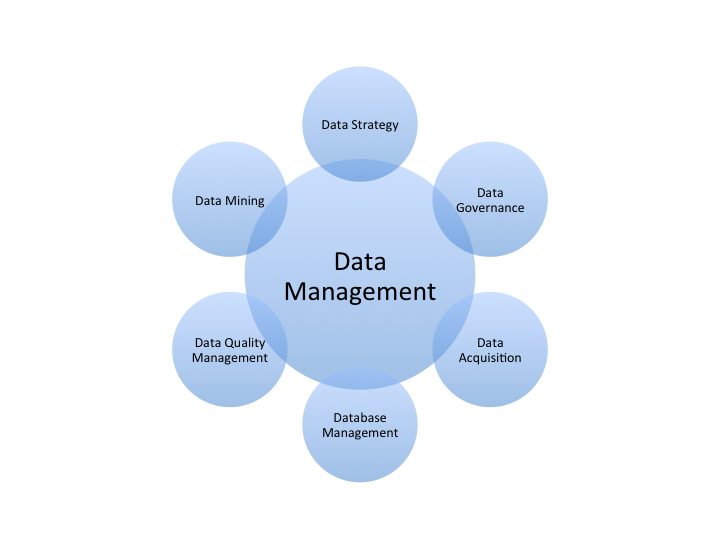
\includegraphics[width=0.8\textwidth]{images/data-management.png}
\centering
\caption{Data Management}
\end{figure}

Big Data is to solve complex enterprise optimization problems. To make the best use of Big Data, we have to recognize that data is a vital corporate asset as data is the lifeblood of the Internet economy. Today organizations rely on data science to make more informed and more effective decisions, which create competitive advantages through innovative products and operational efficiencies.

However, data is firstly a debt. The costs of data acquisition, hardware, software, operation, and talents are very high. Without the right management, it is unlikely for us to effectively extract values from data. To make big data a success, we must have all the disciplines to manage data as a valuable resource. Data management\index{Data!Data management} is much broader than database management. It is a systematic process of capturing, delivering, operating, protecting, enhancing, and disposing of the data cost-effectively, which needs the ever-going reinforcement of plans, policies, programs and practices. 

The ultimate goal of data management is to increase the value proposition of the data. It requires serious and careful consideration and should start with a data strategy that defines a roadmap to meet the business needs in a data-driven approach. To create a data strategy\index{Data!Data strategy}, think carefully of the following questions:
\begin{itemize}
\item What problem do we try to solve? What value can big data bring in? Big data is hot and thus many corporations are hugging it. However, big data for the sake of big data is apparently wrong. Other's use cases do not have to be yours. To glean the value of big data, a deep understanding of your business and problems to solve is essential.
\item Who holds the data, who owns the data, and who can access the data? Data governance\index{Data!Data governance} is a set of processes that ensures that important data assets are formally managed throughout the enterprise. Through data governance, we expect data stewards and data custodians to exercise positive control over the data. Data custodians are responsible for the safe custody, transport, and storage of the data while data stewards are responsible for the management of data elements -- both the content and metadata.
\item What data do we need? It may seem obvious, but it is often simply answered with ``I do not know'' or ``Everything'', which indicates a lack of understanding business practices. Whenever this happens, we should go back to answer the first question again. How to acquire the data? Data may be collected from internal system of records, log files, surveys, or third parties. The transactional systems may be revised to collect necessary data for analytics.
\item Where to store the data and how long to keep them? Due to the variety of data, today's data may be stored in various databases (relational or NoSQL), data warehouses, Hadoop, etc. Today, database management is way beyond relational database administration. Because big data is also fast data, it is impractical to keep all of the data forever. Careful thoughts are needed to determine the lifespan of data.
\item How to ensure the data quality? Junk in, Junk out. Without ensuring the data quality, big data won't bring any values to the business. With the advent of big data, data quality management is both more important and more challenging than ever. 
\item How to analyze and visualize the data? A large number of mathematical models are available for analyzing data. Simply applying mathematical models does not necessarily result in actionable insights. Before talking about your mathematical models, go understand your business and problems. Lead the model with your insights (or {\em a priori} in terms of machine learning) rather than be lead by the uninterpretable numbers of black box models. Besides, visualization is extremely helpful to explore data and present the analytic results as a picture is worth a thousand words.
\item How to manage the complexity? Big data is extremely complicated. To manage the complexity and improve the data management practices, we need to develop the accountability framework to encourage desirable behavior, which is tailored to the organization's business strategies, strengths and priorities.
\end{itemize}

We believe that a good data strategy will emerge after thinking through and answer the above questions.

\chapter[Hadoop]
{Hadoop}
Big data unavoidably needs distributed parallel computing on a cluster of computers. Therefore, we need a distributed data operating system to manage a variety of resources, data, and computing tasks. Today, Apache Hadoop \cite{Hadoop}\index{Hadoop} is the de facto distributed data operating system. Apache Hadoop is an open-source software framework for distributed storage and distributed processing of big data on clusters of commodity hardware. Essentially, Hadoop consists of three parts:
\begin{itemize}
\item HDFS is a distributed high-throughput file system
\item MapReduce for job framework of parallel data processing
\item YARN for job scheduling and cluster resource management
\end{itemize}
The HDFS splits files into large blocks that are distributed (and replicated) among the nodes in the cluster. For processing the data, MapReduce takes advantage of data locality by shipping code to the nodes that have the required data and processing the data in parallel.

\begin{figure}[t]
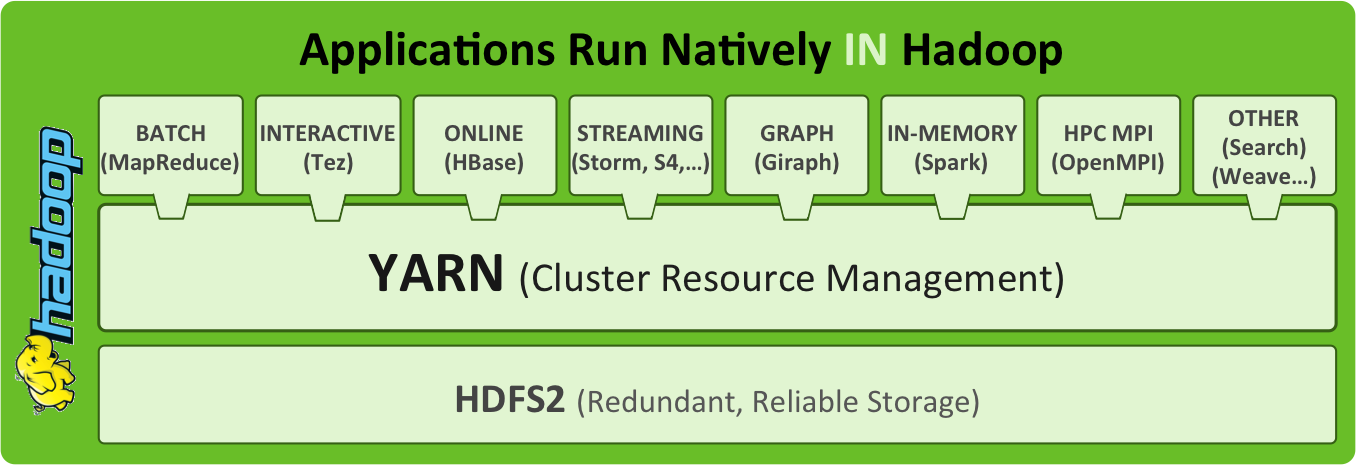
\includegraphics[width=0.8\textwidth]{images/hadoop.png}
\centering
\caption{Hadoop}
%http://4.bp.blogspot.com/-Pm2Q_uyZmPw/U2IvDO7my1I/AAAAAAAABFg/8CAyVoO7F30/s1600/YARN.png
\end{figure}

Originally Hadoop cluster resource management was part of MapReduce because it was the main computing paradigm. Today the Hadoop ecosystem goes beyond MapReduce and includes many additional parallel computing framework, such as Apache Spark, Apache Tez, Apache Storm, etc. So the resource manager, referred to as YARN, was striped out from MapReduce and improved to support other computing framework in Hadoop v2. Now MapReduce is one kind of applications running in a YARN container and other types of applications can be written generically to run on YARN.

\section[HDFS]
{HDFS}
Hadoop Distributed File System (HDFS) \cite{HDFS}\index{HDFS} is a multi-machine file system that runs on top of machines' local file system but appears as a single namespace, accessible through \texttt{hdfs://} URIs. It is designed to reliably store very large files across machines in a large cluster of inexpensive commodity hardware. HDFS closely follows the design of the Google File System (GFS)\index{GFS} \cite{Ghemawat:2003:GFS, McKusick:2009:GEF}.

\subsection{Assumptions}
An HDFS instance may consist of hundreds or thousands of nodes, which are made of inexpensive commodity components that often fail. It implies that some components are virtually not functional at any given time and some will not recover from their current failures. Therefore, constant monitoring, error detection, fault tolerance, and automatic recovery would have to be an integral part of the file system.

HDFS is tuned to support a modest number (tens of millions) of large files, which are typically gigabytes to terabytes in size. Initially, 
HDFS assumes a write-once-read-many access model for files. A file once created, written, and closed need not be changed. This assumption simplifies the data coherency problem and enables high throughput data access. The append operation was added later (single appender only) \cite{HDFS2010:265}.

HDFS applications typically have large streaming access to their datasets. HDFS is mainly designed for batch processing rather than interactive use. The emphasis is on high throughput of data access rather than low latency. 

\subsection{Architecture}
\begin{figure}[t]
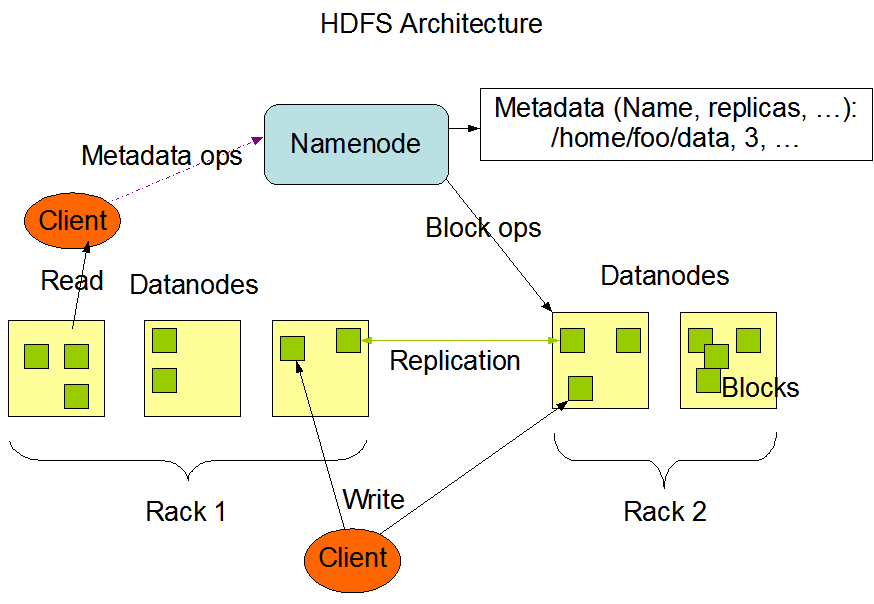
\includegraphics[width=0.8\textwidth]{images/hdfs-architecture.png}
\centering
\caption{HDFS Architecture}
%http://hadoop.apache.org/docs/r1.2.1/images/hdfsarchitecture.gif
\end{figure}

HDFS has a master/slave architecture. An HDFS cluster consists of a single NameNode\index{HDFS!NameNode}, a master server that manages the file system namespace and regulates access to files by clients. In addition, there are a number of DataNodes\index{HDFS!DataNode} that manage storage attached to the nodes that they run on. A typical deployment has a dedicated machine that runs only the NameNode. Each of the other machines in the cluster runs one instance of the DataNode \footnote{Multiple DataNodes on the same machine is possible but rare in production deployments.}.

HDFS supports a traditional hierarchical file organization that consists of directories and files. In HDFS, each file is stored as a sequence of blocks (identified by 64 bit unique id); all blocks in a file except the last one are the same size (typically 64 MB). DataNodes store each block in a separate file  on local file system and provide read/write access. When a DataNode starts up, it scans through its local file system and sends the list of hosted data blocks (called Blockreport) to the NameNode.

For reliability, each block is replicated on multiple DataNodes (three replicas by default). The placement of replicas is critical to HDFS reliability and performance.  HDFS employs a rack-aware replica placement policy to improve data reliability, availability, and network bandwidth utilization. 
When the replication factor is three, HDFS puts one replica on one node in the local rack, another on a different node in the same rack, and the last on a node in a different rack. This policy reduces the inter-rack write traffic which generally improves write performance. Since the chance of rack failure is far less than that of node failure, this policy does not impact data reliability and availability notably.

The NameNode is the arbitrator and repository for all HDFS metadata. The NameNode executes common namespace operations such as create, delete, modify and list files and directories. The NameNode also performs the block management including mapping files to blocks, creating and deleting blocks, and managing replica placement and re-replication. Besides, the NameNode provides DataNode cluster membership by handling registrations and periodic heart beats. But the user data never flows through the NameNode. 

To achieve high performance, the NameNode keeps all metadata in main memory including the file and block namespace, the mapping from files to blocks, and the locations of each block's replicas. The namespace and file-to-block mapping are also kept persistent into the files EditLog\index{HDFS!EditLog} and FsImage\index{HDFS!FsImage} in the local file system of the NameNode. The file FsImage stores the entire file system namespace and file-to-block map. The EditLog is a transaction log to record every change that occurs to file system metadata, e.g. creating a new file and changing the replication factor of a file.
When the NameNode starts up, it reads the FsImage and EditLog from disk, applies all the transactions from the EditLog to the in-memory representation of the FsImage, flushes out the new version of FsImage to disk, and truncates the EditLog.
 
Because the NameNode replays the EditLog and updates the FsImage only during start up, the EditLog could get very large over time and the next restart of NameNode takes longer. To avoid this problem, HDFS has a secondary NameNode that updates the FsImage with the EditLog periodically and keeps the EditLog within a limit. Note that the secondary NameNode is not a standby NameNode. It usually runs on a different machine from the primary NameNode since its memory requirements are on the same order as the primary NameNode.

The NameNode does not store block location information persistently. On startup, the NameNode enters a special state called Safemode\index{HDFS!Safemode} and receives Blockreport messages from the DataNodes. Each block has a specified minimum number of replicas. A block is considered safely replicated when the minimum number of replicas has checked in with the NameNode. After a configurable percentage of safely replicated data blocks checks in with the NameNode (plus an additional 30 seconds), the NameNode exits the Safemode state.

\subsection{Control and Data Flow}
HDFS is designed such that clients never read and write file data through the NameNode. Instead, a client asks the NameNode which DataNodes it should contact using the class ClientProtocol through an RPC connection. Then the client communicates with a DataNode directly to transfer data using the DataTransferProtocol, which is a streaming protocol for performance reasons. Besides, all communication between Namenode and Datanode, e.g. DataNode registration, heartbeat, Blockreport, is initiated by the Datanode, and responded to by the Namenode.

\subsubsection{Read}
First, the client queries the NameNode with the file name, read range start offset, and the range length. The NameNode returns the locations of the blocks of the specified file within the specified range. Especially, DataNode locations for each block are sorted by the proximity to the client. The client then sends a request to one of the DataNodes, most likely the closest one.

\subsubsection{Write}
A client request to create a file does not reach the NameNode immediately. Instead, the client caches the file data into a temporary local file. Once the local file accumulates data worth over one block size, the client contacts the NameNode, which updates the file system namespace and returns the allocated data block location. Then the client flushes the block from the local temporary file to the specified DataNode. When a file is closed, the remaining last block data is transferred to the DataNodes.

\subsection{The Small Files Problem}
Big data but small files (significantly smaller than the block size) implies a lot of files, which creates a big problem for the NameNode \cite{SmallFiles}. Recall that the NameNode holds all the metadata of files and blocks in main memory. Given that each of the metadata object occupies about 150 bytes, the NameNode may host about 10 million files, each using a block, with 3 gigabytes of memory. Although larger memory can push the upper limit higher, large heap is a big challenge for JVM garbage collector.
Furthermore, HDFS is not efficient to read small files because of the overhead of client-NameNode communication, too much disk seeks, and lots of hopping from DataNode to DataNode to retrieve each small file.

In order to reduce the number of files and thus the pressure on the NameNode's memory, Hadoop Archives (HAR files) were introduced. HAR files\index{HDFS!HAR file}, created by \texttt{hadoop archive} \footnote{Archiving does not delete the input files. The user has to do it manually to reduce namespace.} command, are special format archives that contain metadata and data files. The archive exposes itself as a file system layer. All of the original files are visible and accessible through a \texttt{har://} URI. It is also easy to use HAR files as input file system in MapReduce. Note that it is actually slower to read through files in a HAR because of the extra access to metadata.

The SequenceFile\index{HDFS!SequenceFile}, consisting of binary key-value pairs, can also be used to handle the small files problem, by using the filename as the key and the file contents as the value. This works very well in practice for MapReduce jobs. Besides, the SequenceFile supports compression, which reduces disk usage and speeds up data loading in MapReduce. Open source tools exist to convert tar files to SequenceFiles \cite {Tar2Seq}.

The key-value stores, e.g. HBase\index{HBase} and Accumulo\index{Accumulo}, may also be used to reduce file count although they are designed for much more complicated use cases. Compared to SequenceFile, they support random access by keys.

\subsection{HDFS Federation}
The existence of a single NameNode in a cluster greatly simplifies the architecture of the system. However, it also introduces problems. The file count problem, due to the limited memory of NameNode, is an example. A more serious problem is that it proved to be a bottleneck for the clients \cite{McKusick:2009:GEF}. Even though the clients issue few metadata operations to the NameNode, there may be thousands of clients all talking to the NameNode at the same time. With multiple MapReduce jobs, we might suddenly have thousands of tasks in a large cluster, each trying to open a number of files. Given that the NameNode is capable of doing only a few thousand operations a second, it would take a long time to handle all those requests.

Since Hadoop 2.0, we can have two redundant NameNodes in the same cluster in an active/passive configuration with a hot standby. Although this allows a fast failover to a new NameNode for fault tolerance, it does not solve the the performance issue. To partially resolve the scalability problem, the concept of HDFS Federation\index{HDFS!HDFS federation}, was introduced to allow multiple namespaces within a HDFS cluster. In the future, it may also support the cooperation across clusters.

In HDFS Federation, there are multiple independent NameNodes (and thus multiple namespaces). The NameNodes do not require coordination with each other. The DataNodes are used as the common storage by all the NameNodes by registering with and handles commands from all the NameNodes in the cluster. The failure of a NameNode does not prevent the DataNode from serving other NameNodes in the cluster.

Because multiple NameNodes run independently, there may be conflicts of 64 bit block ids generated by different NameNodes. To avoid this problem, a namespace uses one or more block pools, identified by a unique id in a cluster. A block pool belongs to a single namespace and does not cross namespace boundary. The extended block id, a tuple of (Block Pool ID, Block ID), is used for block identification in HDFS Federation.

\subsection{Java API}
HDFS is implemented in Java and provides a native Java API. To access HDFS in other programming languages, Thrift\index{Thrift} \footnote{The Apache Thrift \cite{Thrift} is a software framework for scalable cross-language services development. It combines a software stack with a code generation engine to build services that work efficiently and seamlessly between C++, Java, Python, PHP, Ruby, Erlang, Perl, C\#, Cocoa, JavaScript, Node.js, Smalltalk, OCaml, and Delphi, etc.} bindings are provided for Perl, Python, Ruby and PHP \cite{HdfsThrift}. In what follows, we will discuss how to work with HDFS Java API with a couple of small examples. First of all, we need to add the following dependencies to the project's Maven POM file \cite{Maven}.
\begin{lstlisting}
<dependency>
    <groupId>org.apache.hadoop</groupId>
    <artifactId>hadoop-common</artifactId>
    <version>2.6.0</version>
</dependency>
<dependency>
	<groupId>org.apache.hadoop</groupId>
	<artifactId>hadoop-hdfs</artifactId>
	<version>2.6.0</version>
</dependency>
\end{lstlisting}

The main entry point of HDFS Java API is the abstract class \texttt{FileSystem} in the package \texttt{org.apache.hadoop.fs} that serves as a generic file system representation. \texttt{FileSystem} has various implementations:
\begin{description}
\item[DistributedFileSystem] The implementation of distributed file system. This object is the way end-user code interacts with an HDFS.
\item[LocalFileSystem] The local implementation for small Hadoop instances and for testing.
\item[FTPFileSystem] A FileSystem backed by an FTP client.
\item[S3FileSystem] A block-based FileSystem backed by Amazon S3.
\end{description}

The \texttt{FileSystem} class also serves as a factory for concrete implementations:
\begin{lstlisting}
Configuration conf = new Configuration();
FileSystem fs = FileSystem.get (conf);
\end{lstlisting}
where the \texttt{Configuration} class passes the Hadoop configuration information such as scheme, authority, NameNode host and port, etc. Unless explicitly turned off, Hadoop by default specifies two resources, loaded in-order from the classpath:
\begin{description}
\item[core-default.xml] Read-only defaults for Hadoop.
\item[core-site.xml] Site-specific configuration for a given Hadoop installation.
\end{description}
Applications may add additional resources, which are loaded subsequent to these resources in the order they are added. With \texttt{FileSystem}, one can do common namespace operations, e.g. creating, deleting, and renaming files. We can also query the status of a file such as the length, block size, block locations, permission, etc. To read or write files, we need to use the classes \texttt{FSDataInputStream} and \texttt{FSDataOutputStream}. In the following example, we develop two simple functions to copy a local file into/from HDFS. For simplicity, we do not check the file existence or any I/O errors. Note that \texttt{FileSystem} does provide several utility functions for copying files between local and distributed file systems.

\begin{lstlisting}
/** Copy a local file to HDFS */
public void copyFromLocal(String src, String dst) throws IOException {
 
  Configuration conf = new Configuration();
  FileSystem fs = FileSystem.get(conf);
  
  // The Path object represents a file or directory in HDFS.
  FSDataOutputStream out = fs.create(new Path(dst));
  InputStream in = new BufferedInputStream(new FileInputStream(new File(src)));
 
  byte[] b = new byte[1024];
  int numBytes = 0;
  while ((numBytes = in.read(b)) > 0) {
    out.write(b, 0, numBytes);
  }
 
  in.close();
  out.close();
  fs.close();
}

/** Copy an HDFS file to local file system */
public void copyToLocal(String src, String dst) throws IOException {
 
  Configuration conf = new Configuration();
  FileSystem fs = FileSystem.get(conf);
 
  FSDataInputStream in = fs.open(new Path(src));
  OutputStream out = new BufferedOutputStream(new FileOutputStream(new File(dst)));
  byte[] b = new byte[1024];
  int numBytes = 0;
  while ((numBytes = in.read(b)) > 0) {
    out.write(b, 0, numBytes);
  }
 
  in.close();
  out.close();
  fs.close();
}
\end{lstlisting}

In the example, we use the method \texttt{FileSystem.create} to create an \texttt{FSDataOutputStream} at the indicated \texttt{Path}. If the file exists, it will be overwritten by default. The \texttt{Path} object is used to locate a file or directory in HDFS. \texttt{Path} is really a URI. For HDFS, it takes the format of \texttt{hdfs://host: port/location}. To read an HDFS file, we use the method \texttt{FileSystem.open} that returns an \texttt{FSDataInputStream} object. The rest of example is just as the regular Java I/O stream operations.

\subsection[Data Ingestion]
{Data Ingestion}

Today, most data are generated and stored out of Hadoop, e.g. relational databases, plain files, etc. Therefore, data ingestion is the first step to utilize the power of Hadoop. To move the data into HDFS, we do not have to do the low level programming as the previous example. Various utilities have been developed to move data into Hadoop.

\subsubsection{Batch Data Ingestion}
The File System Shell\index{HDFS!File System Shell} \cite{HdfsShell} includes various shell-like commands, including \texttt{copyFromLocal} and \texttt{copyToLocal}, that directly interact with the HDFS as well as other file systems that Hadoop supports. Most of the commands in File System Shell behave like corresponding Unix commands. When the data files are ready in local file system, the shell is a great tool to ingest data into HDFS in batch. In order to stream data into Hadoop for real time analytics, however, we need more advanced tools, e.g. Apache Flume and Apache Chukwa. 

\subsubsection{Streaming Data Ingestion}
Apache Flume\index{Flume} \cite{Flume} is a distributed, reliable, and available service for efficiently collecting, aggregating, and moving large amounts of log data into HDFS. It has a simple and flexible architecture based on streaming data flows; and robust and fault tolerant with tunable reliability mechanisms and many failover and recovery mechanisms. It uses a simple extensible data model that allows for online analytic application. Flume employs the familiar producer-consumer model. \texttt{Source} is the entity through which data enters into Flume. Sources either actively poll for data or passively wait for data to be delivered to them. On the other hand, \texttt{Sink} is the entity that delivers the data to the destination. Flume has many built-in sources (e.g. log4j and syslogs) and sinks (e.g. HDFS and HBase). \texttt{Channel} is the conduit between the Source and the Sink. Sources ingest events into the channel and the sinks drain the channel. Channels allow decoupling of ingestion rate from drain rate. When data are generated faster than what the destination can handle, the channel size increases.

Apache Chukwa\index{Chukwa} \cite{Chukwa} is devoted to large-scale log collection and analysis, built on top of MapReduce framework. Beyond data ingestion, Chukwa also includes a flexible and powerful toolkit for displaying monitoring and analyzing results. Different from Flume, Chukwa is not a a continuous stream processing system but a mini-batch system.

Apache Kafka\index{Kafka} \cite{Kafka} and Apache Storm\index{Storm} \cite{Storm} may also be used to ingest streaming data into Hadoop although they are mainly designed to solve different problems. Kafka is a distributed publish-subscribe messaging system. It is designed to provide high throughput persistent messaging that's scalable and allows for parallel data loads into Hadoop. Storm is a distributed realtime computation system for use cases such as realtime analytics, online machine learning, continuous computation, etc.

\subsubsection{Structured Data Ingestion}
Apache Sqoop\index{Sqoop} \cite{Sqoop} is a tool designed to efficiently transfer data between Hadoop and relational databases. We can use Sqoop to import data from a relational database table into HDFS. The import process is performed in parallel and thus generates multiple files in the format of delimited text, Avro, or SequenceFile. Besides, Sqoop generates a Java class that encapsulates one row of the imported table, which can be used in subsequent MapReduce processing of the data. Moreover, Sqoop can export the data (e.g. the results of MapReduce processing) back to the relational database for consumption by external applications or users.

\section[MapReduce]
{MapReduce}
\index{MapReduce}Distributed parallel computing is not new. Supercomputers have been using MPI\index{MPI} \cite{Forum:1994:MMI} for years for complex numerical computing. Although MPI provides a comprehensive API for data transfer and synchronization, it is not very suitable for big data. Due to the large data size and shared-nothing architecture for scalability, data distribution and I/O are critical to big data analytics while MPI almost ignores it \footnote{MPI-I/O \cite{Gropp:1999:UMA} was added into MPI-2 but it is not easy to use and difficult to achieve good performance.}. On the other hand, many big data analytics are conceptually straightforward and does not need very complicated communication and synchronization mechanism. Based on these observations, Google invented MapReduce \cite{Dean:2008:MSD} to deal the issues of how to parallelize the computation, distribute the data, and handle failures.

\subsection{Overview}
In a shared-nothing distributed computing environment, a computation is much more efficient if it is executed near the data it operates on. This is especially true when the size of the data set is huge as it minimizes network traffic and increases the overall throughput of the system. Therefore, it is often better to migrate the computation closer to where the data is located rather than moving the data to where the application is running. With GFS/HDFS, MapReduce provides such a parallel programming framework.

Inspired by the \texttt{map} and \texttt{reduce}\footnote{Also frequently referred as \texttt{fold}.} functions commonly used in functional programming, a MapReduce program is composed of a Map()\index{MapReduce!Map} procedure that performs transformation and a Reduce()\index{MapReduce!Reduce} procedure that takes the shuffled output of Map as input and performs a summarization operation. More specifically, the user-defined Map function processes a key-value pair to generate a set of intermediate key-value pairs, and the Reduce function aggregates all intermediate values associated with the same intermediate key.

MapReduce applications are automatically parallelized and executed on a large cluster of commodity machines. During the execution, the Map invocations are distributed across multiple machines by automatically partitioning the input data into a set of M splits. The input splits can be processed in parallel by different machines. Reduce invocations are distributed by partitioning the intermediate key space into R pieces using a partitioning function. The number of partitions and the partitioning function are specified by the user. Besides partitioning the input data and running the various tasks in parallel, the framework also manages all communications and data transfers, load balance, and fault tolerance.

MapReduce provides programmers a really simple parallel computing paradigm. Because of automatic parallelization, no explicit handling of data transfer and synchronization in programs, and no deadlock, this model is very attractive. MapReduce is also designed to process very large data that is too big to fit into the memory (combined from all nodes). To achieve that, MapReduce employs a data flow model, which also provides a simple I/O interface to access large amount of data in distributed file system. It also exploits data locality for efficiency. In most cases, we do not need to worry about I/O at all.

\subsection{Data Flow}
\begin{figure}[t]
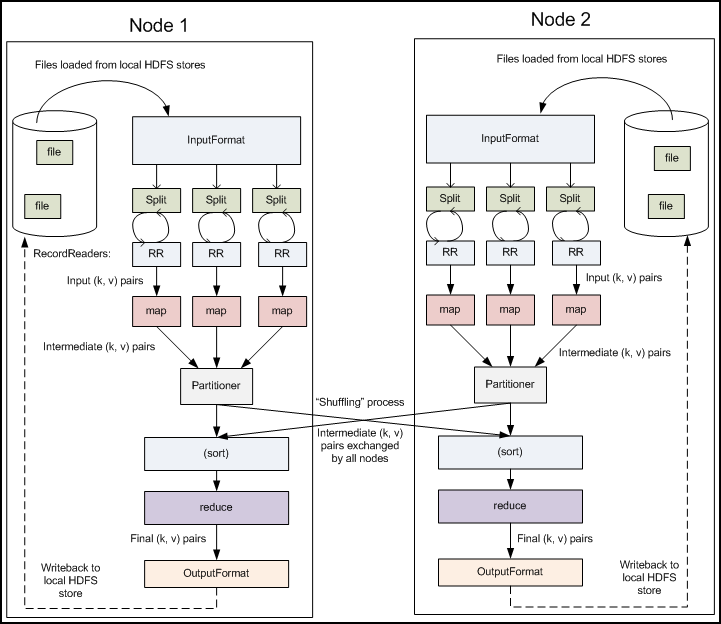
\includegraphics[width=0.8\textwidth]{images/MapReduce.png}
\centering
\caption{MapReduce Data Flow}
%http://4.bp.blogspot.com/-2S6IuPD71A8/TZiNw8AyWkI/AAAAAAAAB0k/tS5QTP9SzHA/s1600/Detailed%2BHadoop%2BMapreduce%2BData%2BFlow.png
\end{figure}

For a given task, the MapReduce system runs as follows
\begin{description}
\item[Prepare the Map() input]
The system splits the input files into M pieces and then starts up M Map workers on a cluster of machines.
\item[Run the user-defined Map() code]
The Map worker parses key-value pairs out of the assigned split and passes each pair to the user-defined Map function. The intermediate key-value pairs produced by the Map function are buffered in memory. Periodically, the buffered pairs are written to local disk, partitioned into R regions for sharding purposes by the partitioning function (called partitioner\index{MapReduce!Partitioner}) that is given the key and the number of reducers R and returns the index of the desired reducer.
\item[Shuffle the Map output to the Reduce processors]
\index{MapReduce!Shuffle}When ready, a reduce worker reads remotely the buffered data from the local disks of the map workers. When a reduce worker has read all intermediate data, it sorts the data by the intermediate keys so that all occurrences of the same key are grouped together. Typically many different keys map to the same reduce task.
\item[Run the user-defined Reduce() code]
The reduce worker iterates over the sorted intermediate data and for each unique intermediate key encountered, it passes the key and the corresponding set of intermediate values to the user's Reduce function.
\item[Produce the final output]
The final output is available in the R output files (one per reduce task).
\end{description}
Optionally, a combiner\index{MapReduce!Combiner} can be used between map and reduce as an optimization. The combiner function runs on the output of the map phase and is used as a filtering or an aggregating step to lessen the data that are being passed to the reducer. In most of the cases the reducer class is set to be the combiner class so that we can save network time. Note that this works only if reduce function is commutative and associative.

In practice, one should pay attention to the task granularity, i.e. the number of map tasks M and the number of reduce tasks R. In general, M should be much larger than the number of nodes in cluster, which improves load balancing and speeds recovery from worker failure. The right level of parallelism for maps seems to be around 10-100 maps per node (maybe more for very cpu light map tasks). Besides, the task setup takes awhile. On a Hadoop cluster of 100 nodes, it takes 25 seconds until all nodes are executing the job. So it is best if the maps take at least a minute to execute. In Hadoop, one can call \texttt{JobConf.setNumMapTasks(int)} to set the number of map tasks. Note that it only provides a hint to the framework.

The number of reducers is usually a small multiple of the number of nodes. The right factor number seems to be 0.95 for well-balanced data (per intermediate key) or 1.75 otherwise for better load balancing. Note that we reserve a few reduce slots for speculative tasks and failed tasks. We can set the number of reduce tasks by \texttt{JobConf.setNumReduceTasks(int)} in Hadoop and the framework will honor it. It is fine to set R to zero if no reduction is desired.

\subsection{Secondary Sorting}
The output of Mappers is firstly sorted by the intermediate keys. However, we do want to sort the intermediate values (or some fields of intermediate values) sometimes, e.g. calculating the stock price moving average where the key is the stock ticker and the value is a pair of timestamp and stock price. If the values of a given key are sorted by the timestamp, we can easily calculate the moving average with a sliding window over the values. This problem is called secondary sorting.

A direct approach to secondary sorting is for the reducer to buffer all of the values for a given key and do an in-memory sort. Unfortunately, it may cause the reducer to run out of memory.

Alternatively, we may use a composite key that has multiple parts. In the case of calculating moving average, we may create a composite key of (ticker, timestamp) and also provide a customized sort comparator (subclass of \texttt{WritableComparator}) that compares ticker and then timestamp.
To ensure only the ticker (referred as natural key) is considered when determining which reducer to send the data to, we need to write a custom partitioner (subclass of \texttt{Partitioner}) that is solely based on the natural key.
Once the data reaches a reducer, all data is grouped by key. Since we have a composite key, we need to make sure records are grouped solely by the natural key by implementing a group comparator (another subclass of \texttt{WritableComparator}) that considers only the natural key.

\subsection{Examples}
Hadoop implements MapReduce in Java. To create a MapReduce program, please add the following dependencies to the project's Maven POM file.

\begin{lstlisting}
<dependency>
    <groupId>org.apache.hadoop</groupId>
    <artifactId>hadoop-common</artifactId>
    <version>2.6.0</version>
</dependency>
<dependency>
    <groupId>org.apache.hadoop</groupId>
    <artifactId>hadoop-mapreduce-client-core</artifactId>
    <version>2.6.0</version>
</dependency>
<dependency>
    <groupId>org.apache.hadoop</groupId>
    <artifactId>hadoop-hdfs</artifactId>
    <version>2.6.0</version>
</dependency>
\end{lstlisting}

\subsubsection{Sort}

The essential part of the MapReduce framework is a large distributed sort. So we just let the framework do the job in this case while the map is as simple as emitting the sort key and original input. In the below example, we just assume the input key is the sort key. The reduce operator is an identity function.

\begin{lstlisting}
public class SortMapper extends Mapper<IntWritable, Text, IntWritable, Text> {

  public void map(IntWritable key, Text value, Context context)
    throws IOException, InterruptedException {
    context.write(key, value);
  }
}

public class SortReducer extends Reducer<IntWritable, Text, IntWritable, Text> {

  public void reduce(IntWritable key, Iterable<Text> values, Context context)
    throws IOException, InterruptedException {
    for (Text value : values) {
      context.write(key, value);
    }
  }
}
\end{lstlisting}

Although this example is extremely simple, there are many important classes to understand. The MapReduce framework takes key-value pairs as the input and produces a new set of key-value pairs (maybe of different types).
The key and value classes have to be serializable by the framework and hence need to implement the \texttt{Writable} interface. Additionally, the key classes have to implement the \texttt{WritableComparable} interface to facilitate sorting by the framework.

The \texttt{map} method of \texttt{Mapper} implementation processes one key-value pair in the input split at a time. The \texttt{reduce} method of \texttt{Reducer} implementation is called once for each intermediate key and associate group of values. In this case, we do not have to override the \texttt{map} and \texttt{reduce} methods because the default implementation is actually an identity function. The sample code is mainly to show the interface. Both \texttt{Mapper} and \texttt{Reducer} emit their output through the \texttt{Context} object provided by the framework.

To submit a MapReduce job to Hadoop, we need to do the below steps. First, the application describes various facets of the job via \texttt{Job} object. \texttt{Job} is typically used to specify the \texttt{Mapper}, \texttt{Reducer}, \texttt{InputFormat}, \texttt{OutputFormat} implementations, the directories of input files and the location of output files.
Optionally, one may specify advanced facets of the job such as the Combiner, Partitioner, Comparator, and DistributedCache, etc. Then the application submits the job to the cluster by the method \texttt{waitForCompletion(boolean verbose)}  and wait for it to finish.
\texttt{Job} also allows the user to control the execution and query the state.
\begin{lstlisting}
public class MapReduceSort {
  public static void main(String[] args) throws Exception {
    Configuration conf = new Configuration();
    Job job = Job.getInstance(conf, "sort");
    job.setJarByClass(MapReduceSort.class);
    job.setMapperClass(SortMapper.class);
    job.setReducerClass(SortReducer.class);
    job.setOutputKeyClass(IntWritable.class);
    job.setOutputValueClass(Text.class);

    FileInputFormat.addInputPath(job, new Path(args[0]));
    FileOutputFormat.setOutputPath(job, new Path(args[1]));

    System.exit(job.waitForCompletion(true) ? 0 : 1);
  }
}
\end{lstlisting}
\subsubsection{Grep}

The map function emits a line if it matches a given pattern. The reduce part is not necessary in this case and we can simply set the number of reduce tasks zero (\texttt{job.setNumReduceTasks(0)}). Note that the \texttt{Mapper} implementation also overrides the \texttt{setup} method, which will be called once at the beginning of the task. In this case, we use it to set the search pattern from the job configuration. This is also a good example of passing small configuration data to MapReduce tasks. To pass large amount of read-only data to tasks, DistributedCache is preferred and will be discussed later in the case of Inner Join. Similar to \texttt{setup}, one may also overrides the \texttt{cleanup} method, which will be called once at the end of the task.

\begin{lstlisting}
public class GrepMapper<K> extends Mapper<K, Text, K, Text> {

  public static String PATTERN = "mapper.pattern";
  private Pattern pattern;

  // Setup the match pattern from job context.
  // Called once at the beginning of the task.
  public void setup(Context context) {
    Configuration conf = context.getConfiguration();
    pattern = Pattern.compile(conf.get(PATTERN));
  }

  public void map(K key, Text value, Context context)
    throws IOException, InterruptedException {
    if (pattern.matcher(value.toString()).find()) {
      context.write(key, value);
    }
  }
}
\end{lstlisting}
In a relational database, one can achieve this by the following simple query in SQL.

\lstset{language=SQL}
\begin{lstlisting}
SELECT * FROM T_KV WHERE value LIKE '%XYZ%';
\end{lstlisting}
Although this query requires a full table scan, a parallel DMBS can easily outperformance MapReduce in this case. It is because the setup cost of MapReduce is high.
The performance gap will be much larger in case that an index can be used such as

\begin{lstlisting}
SELECT * FROM T_PERSON WHERE age > 30;
\end{lstlisting}
 

\subsubsection{Aggregation}

Aggregation is a simple analytic calculation such as counting the number of access or users from different countries. WordCount, the ``hello world'' program in the MapReduce world, is an example of aggregation. WordCount simply counts the number of occurrences of each word in a given input set. The Mapper splits the input line into words  and emits a key-value pair of \textless word, 1\textgreater. The Reducer just sums up the values. For the sample code, please refer Hadoop's MapReduce Tutorial \cite{MapReduceTutorial}.

For SQL, aggregation simply means GROUP BY such as the following example:
\begin{lstlisting}
SELECT country, count(*) FROM T_WEB_LOG GROUP BY country;
\end{lstlisting}
With a combiner, the aggregation in MapReduce works pretty much same as in a parallel DBMS. Of course, a DBMS can still benefit a lot from an index on the group by field.

\subsubsection{Inner Join}

An inner join operation combines two data sets, A and B, to produce a third one containing all record pairs from A and B with matching attribute value. The sort-merge join algorithm and hash-join algorithm are two common alternatives to implement the join operation in a parallel data flow environment \cite{DeWitt:1992:PDS}. In sort-merge join, both A and B are sorted by the join attribute and then compared in sorted order. The matching pairs are inserted into the output stream. The hash-join first prepares a hash table of the smaller data set with the join attribute as the hash key. Then we scan the larger dataset and find the relevant rows from the smaller dataset by searching the hash table.

There are several ways to implement join in MapReduce, e.g. reduce-side join and map-side join. The reduce-side join is a straightforward approach that takes advantage of that identical keys are sent to the same reducer. In the reduce-side join, the output key of Mapper has to be the join key so that they reach the same reducer. The Mapper also tags each dataset with an identity to differentiate them in the reducer. With secondary sorting on the dataset identity, we ensure the order of values sent to the reducer, which generates the matched pairs for each join key.
Because two datasets are usually in different formats, we can use the class \texttt{MultipleInputs} to setup different \texttt{InputFormat} and \texttt{Mapper} for each input path. The reduce-side join belongs to the sort-merge join family and scales very well for large datasets. However, it may be less efficient in the case of data skew where a dataset is significantly smaller than the other.

If one dataset is small enough to fit into the memory, we may use the memory-based map-side join. In this approach, the Mappers side-load the smaller dataset and build a hash table of it during the setup, and process the rows of the larger dataset one-by-one in the map function. To efficiently load the smaller dataset in every Mapper, we should use the \texttt{DistributedCache}\index{MapReduce!DistributedCache}. The \texttt{DistributedCache} is a facility to cache application-specific large, read-only files. 
An application specifies the files to be cached by \texttt{Job.addCacheFile(URI)}. The MapReduce framework will copy the necessary files on to the slave node before any tasks for the job are executed on that node. This is much more efficient than that copying the files for each Mapper. Besides, we can declare the hash table as a static field so that the
tasks running successively in a JVM will share the data using the task JVM reuse feature. Thus, we only need to load the data only once for each JVM.

The above map-side join is fast but only works when the smaller dataset fits in the memory. To avoid this pitfall, we can use the multi-phrase map-side join. First we run a MapReduce job on each dataset that uses the join attribute as the Mapper's and Reducer's output key and have the same number of reducers for all datasets. In this way, all datasets are sorted by the join attribute and have the same number of partitions. In second phrase, we use \texttt{CompositeInputFormat} as the input format. The \texttt{CompositeInputFormat} performs joins over a set of data sources sorted and partitioned the same way, which is guaranteed by the first phrase. So the records are already merged before they reach the Mapper, which simplify outputs the joins to the stream.

Because the join implementation is fairly complicated, we will not show the sample code here. In practice, one should use higher level tools such as Hive or Pig to join data sets rather than reinventing the wheel.

In practice, join, aggregation, and sort are frequently used together, e.g. finding the client of the ad that generates the most revenue (or clicks) during a period. In MapReduce, this has to be done in multiple phases. The first phrase filters the data base on the click timestamp and joins the client and click log datasets. The second phrase does the aggregation on the output of join and the third one finishes the task by sorting the output of aggregation. 

Various benchmarks shows that parallel DBMSs are way faster than MapReduce for joins \cite{Pavlo:2009:CAL}. Again an index on the join key is very helpful. But more importantly, joins can be done locally on each node if both tables are partitioned by the join key so that no data transfer is needed before the join.

\subsubsection{K-Means Clustering}

The k-means clustering is a simple and widely used method that partitions data into k clusters in which each record belongs to the cluster with the nearest center, serving as a prototype of the cluster \cite{Jain:1988:ACD}. The most common algorithm for k-means clustering is Lloyd's algorithm that iteratively proceeds by alternating between two steps. The assignment step assigns each sample to the cluster of nearest mean. The update step calculates the new means to be the centroids of the samples in the new clusters. The algorithm converges when the assignments no longer change. The algorithm can be naturally implemented in the MapReduce framework where each iteration will be a MapReduce job.
\begin{description}
\item[Input] The data files as regular MapReduce input and cluster center files side-loaded by DistributedCache. Initially, the cluster centers may be random selected.
\item[Map] With side-loaded cluster centers, each sample input is mapped to a cluster of nearest mean. The emitted key-value pair is \textless cluster id, sample vector\textgreater.
\item[Combine] In order to reduce the data passed to the reducer, we may have a combiner that aggregates samples belonging to the same cluster.
\item[Reduce] The reduce tasks recalculate the new means of clusters as the centroids of samples in the new clusters. The output of new cluster means will be used as the input to next iteration.
\item[Iterate] This process is repeated until the algorithm converges or reaches the maximum number of iterations.
\item[Output] Runs a map only job to output the cluster assignment.
\end{description}

Such an implementation is very scalable. it can handle very large data size, which may be even larger than the combined memory of the cluster. On the other hand, it is not very efficient because the input data have to been read again and again for each iteration. This is a general performance issue for MapReduce to implement iterative algorithms.
 
\subsection{Shortcomings}
The above examples show that MapReduce is capable of a variety of tasks. On the other hand, they also demonstrate several drawbacks of MapReduce.
\subsubsection{Performance}
MapReduce provides a scalable programming model on large clusters. However, it is not guaranteed to be fast due to many reasons:
\begin{itemize}
\item Even though Hadoop now reuses JVM instances for map and reduce tasks, the startup time is still significant on large clusters. The high startup cost means that MapReduce is mainly suitable for long run batch jobs.
\item The communication between map and reduce tasks always are done by remote file access, which actually often dominates the computation cost. Such a pulling strategy is great for fault tolerance, but it results in low performance compared to the push mechanism. Besides there could be M * R intermediate files. Given large M and R, it is certainly a challenge for underlying file system. With multiple reducers running simultaneously, it is highly likely that some of them will attempt to read from the same map node at the same time, inducing a large number of disk seeks and slowing the effective disk transfer rate.
\item Iterative algorithms perform poorly on MapReduce because of reading input data again and again. Data also must be materialized and replicated on the distributed file system between successive jobs.
\end{itemize}
\subsubsection{Low Level Programming Interface}
A major goal of MapReduce is to provide a simple programming model that application developers need only to write the map and reduce parts of the program. However, practical programmers have to take care of a lot things such as input/output format, partition functions, comparison functions, combiners, and job configuration to achieve good performance. As shown in the example, even a very simple grep MapReduce program is fairly long. On the other hand, the same query in SQL is much shorter and cleaner.

MapReduce is independent of the underlying storage system. It's application developers' duty to organize data such as building and using any index, partitioning and collocating related data sets, etc. Unfortunately, these are not easy tasks in the context of HDFS and MapReduce.

\subsubsection{Limited Parallel Computing Model}
The simple computing model of MapReduce brings us no explicit handling of data transfer and synchronization in programs, and no deadlock. But it is a limited parallel computing model, essentially a scatter-gather processing model. For non-trivial algorithms, programmers try hard to ``MapReducize'' them, often in a non-intuitive way.

After years of practice, the community has realized these problems and tries to address them in different ways. For example, Apache Spark aims on the speed by keeping data in memory. Apache Pig provides a DSL and Hive provides a SQL dialect on the top of MapReduce to ease the programming. Google Dremel and Cloudera Impala target on interactive analysis with SQL queries. Microsoft Dryad/Apache Tez provides a more general parallel computing framework that models computations in DAGs. Google Pregel and Apache Giraph concerns computing problems on large graphs. Apache Storm focuses on real time event processing. We will look into all of them in the rest of book. First, we will check out Tez and Spark in this chapter.

\section[Tez]
{Tez}
\index{Tez}
MapReduce provides a scatter-gather parallel computing model, which is very limited. Dryad, a research project at Microsoft Research, attempted to support a more general purpose runtime for parallel data processing\index{Dryad} \cite{Isard:2007:DDD}. A Dryad job is a directed acyclic graph (DAG) where each vertex is a program and edges represent data channels (files, TCP pipes, or shared-memory FIFOs). The DAG defines the data flow of the application, and the vertices of the graph defines the operations that are to be performed on the data. It is a logical computation graph that is automatically mapped onto physical resources by the runtime. Dryad includes a domain-specific language, in C++ as a library using a mixture of method calls and operator overloading, that is used to create and model a Dryad execution graph. Dryad is notable for allowing graph vertices to use an arbitrary number of inputs and outputs, while MapReduce restricts all computations to take a single input set and generate a single output set. Although Dryad provides a nice alternative to MapReduce, Microsoft discontinued active development on Dryad, shifting focus to the Apache Hadoop framework in October 2011.

Interestingly, the Apache Hadoop community recently picked up the idea of Dryad and developed Apache Tez \cite{Tez, TezTutorial}, a new runtime framework on YARN, during the Stinger initiative\index{Stinger} of Hive\index{Hive} \cite{Stinger}. Similar to Dryad, Tez is an application framework which allows for a complex directed-acyclic-graph of tasks for processing data. Edges of data flow graph determine how the data is transferred and the dependency between the producer and consumer vertices. Edge properties enable Tez to instantiate user tasks, configure their inputs and outputs, schedule them appropriately and define how to route data between the tasks. The edge properties include:
\begin{description}
\item[Data movement] determines routing of data between tasks.
\begin{itemize}
\item One-To-One: Data from the $i^{th}$ producer task routes to the $i^{th}$ consumer task.
\item Broadcast: Data from a producer task routes to all consumer tasks.
\item Scatter-Gather: Producer tasks scatter data into shards and consumer tasks gather the shards. The $i^{th}$ shard from all producer tasks routes to the $i^{th}$ consumer task.
\end{itemize}
\item[Scheduling] determines when a consumer task is scheduled.
\begin{itemize}
\item Sequential: Consumer task may be scheduled after a producer task completes.
\item Concurrent: Consumer task must be co-scheduled with a producer task.
\end{itemize}
\item[Data source] determines the lifetime/reliability of a task output.
\begin{itemize}
\item Persisted: Output will be available after the task exits. Output may be lost later on.
\item Persisted-Reliable: Output is reliably stored and will always be available.
\item Ephemeral: Output is available only while the producer task is running.
\end{itemize}
\end{description}
For example, MapReduce would be expressed with the scatter-gather, sequential and persisted edge properties. 

The vertex in the data flow graph defines the user logic that transforms the data. Tez models each vertex as a composition of Input, Processor and Output modules. Input and Output determine the data format and how and where it is read/written. An input represents a pipe through which a processor can accept input data from a data source such as HDFS or the output generated by another vertex, while an output represents a pipe through which a processor can generate output data for another vertex to consume or to a data sink such as HDFS. Processor holds the data transformation logic, which consumes one or more Inputs and produces one or more Outputs.

The Tez runtime expands the logical graph into a physical graph by adding parallelism at the vertices, i.e. multiple tasks are created per logical vertex to perform the computation in parallel. A logical edge in a DAG is also materialized as a number of physical connections between the tasks of two connected vertices. Tez also supports pluggable vertex management modules to collect information from tasks and change the data flow graph at runtime to optimize performance and resource usage.

With Tez, Apache Hive is now able to process data in a single Tez job, which may take multiple MapReduce jobs. If the data processing is too complicated to finish in a single Tez job, Tez session can encompass multiple jobs by leveraging common services. This provides additional performance optimizations.
\begin{figure}[t]
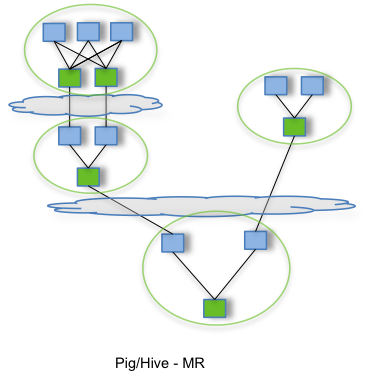
\includegraphics[width=0.4\textwidth]{images/PigHive_MR.png}
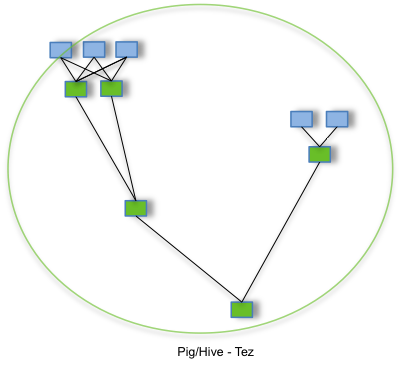
\includegraphics[width=0.4\textwidth]{images/PigHive_Tez.png}
\centering
\caption{Pig/Hive on MapReduce vs Tez}
%http://tez.apache.org/images/PigHiveQueryOnMR.png
%http://tez.apache.org/images/PigHiveQueryOnTez.png
\end{figure}

Like MapReduce, Tez is still a lower-level programming model. To obtain good performance, the developer must understand the structure of the computation and the organization and properties of the system resources. 

\section[YARN]
{YARN}
\index{YARN} Originally, Hadoop was restricted mainly to the paradigm MapReduce, where the resource management is done by JobTracker and TaskTacker.
The JobTracker farms out MapReduce tasks to specific nodes in the cluster, ideally the nodes that have the data, or at least are in the same rack. A TaskTracker is a node in the cluster that accepts tasks - Map, Reduce and Shuffle operations - from a JobTracker. Because Hadoop has stretched beyond MapReduce (e.g. HBase, Storm, etc.), Hadoop now architecturally decouples the resource management features from the programming model of MapReduce, which makes Hadoop clusters more generic. The new resource manager is referred to as MapReduce 2.0 (MRv2) or YARN \cite{YARN2011:279}. Now MapReduce is one kind of applications running in a YARN container and other types of applications can be written generically to run on YARN.

YARN employs a master-slave model and includes several components:
\begin{itemize}
\item The global Resource Manager is the ultimate authority that arbitrates resources among all applications in the system.
\item The per-application Application Master negotiates resources from the Resource Manager and works with the Node Managers to execute and monitor the component tasks.
\item The per-node slave Node Manager\index{YARN!Node manager} is responsible for launching the applications' containers, monitoring their resource usage and reporting to the Resource Manager.
\end{itemize}

\begin{figure}[t]
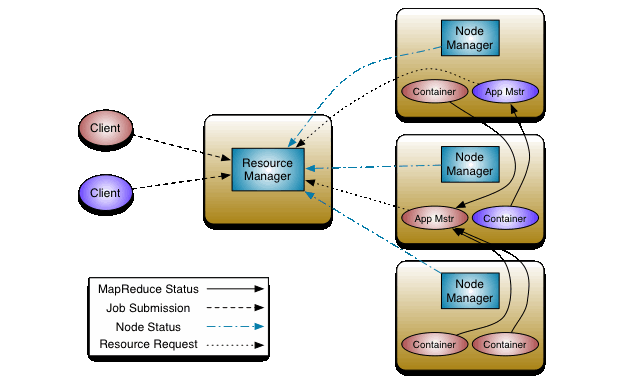
\includegraphics[width=0.8\textwidth]{images/yarn-architecture.png}
\centering
\caption{YARN Architecture}
%http://hadoop.apache.org/docs/current/hadoop-yarn/hadoop-yarn-site/yarn_architecture.gif
\end{figure}

The Resource Manager\index{YARN!Resource manager}, consisting of Scheduler\index{YARN!Scheduler} and Application Manager\index{YARN!Application manager}, is the central authority that arbitrates resources among various competing applications in the cluster.
The Scheduler is responsible for allocating resources to the various running applications subject to the constraints of capacities, queues etc.
The Application Manager is responsible for accepting job-submissions, negotiating the first container for executing the application specific Application Master and provides the service for restarting the Application Master container on failure.

The Scheduler uses the abstract notion of a Resource Container\index{YARN!Resource container} which incorporates elements such as memory, CPU, disk, network etc. Initially, YARN uses the memory-based scheduling. Each node is configured with a set amount of memory and applications  request containers for their tasks with configurable amounts of memory. Recently, YARN added CPU as a resource in the same manner. Nodes are configured with a number of ``virtual cores'' (vcores) and applications give a vcore number in the container request.

The Scheduler has a pluggable policy plug-in, which is responsible for partitioning the cluster resources among the various queues, applications etc. For example, the Capacity Scheduler\index{YARN!Scheduler!Capacity scheduler} is designed to maximize the throughput and the utilization of shared, multi-tenant clusters.
Queues\index{YARN!Queue} are the primary abstraction in the Capacity Scheduler. The capacity of each queue specifies the percentage of cluster resources that are available for applications submitted to the queue. Furthermore, queues can be set up in a hierarchy. YARN also sports a Fair Scheduler\index{YARN!Scheduler!Fair scheduler}  that tries to assign resources to applications such that all applications get an equal share of resources over time on average using dominant resource fairness \cite{Ghodsi:2011:DRF}.

The protocol between YARN and applications is as follows. First an Application Submission Client communicates with the Resource Manager to acquire a new Application Id. Then it submit the Application to be run by providing sufficient information (e.g. the local files/jars, command line, environment settings, etc.) to the Resource Manager to launch the Application Master. 
The Application Master is then expected to register itself with the Resource Manager and request for and receive containers. After a container is allocated to it, the Application Master communicates with the Node Manager to launch the container for its task by specifying the launch information such as command line specification, environment, etc. The Application Master also handles failures of job containers. Once the task is completed, the Application Master signals the Resource Manager.

As the central authority of the YARN cluster, the Resource Manager is also the single point of failure (SPOF\index{SPOF}). To make it fault tolerant, an Active/Standby architecture can be employed since Hadoop 2.4. Multiple Resource Manager instances (listed in the configuration file yarn-site.xml) can be brought up but only one instance is Active at any point of time while others are in Standby mode. 
When the Active goes down or becomes unresponsive, another Resource Manager is automatically elected by a ZooKeeper-based method to be the Active. ZooKeeper\index{ZooKeeper} is a replicated CP key-value store, which we will discuss in details later. Clients, Application Masters and Node Managers try connecting to the Resource Managers in a round-robin fashion until they hit the new Active. 

\chapter[Spark]
{Spark}
\index{Spark} Although MapReduce is great for large scale data processing, it is not friendly for iterative algorithms or interactive analytics because the data have to be repeatedly loaded for each iteration or be materialized and replicated on the distributed file system between successive jobs. Apache Spark \cite{Zaharia:2010:SCC, Zaharia:2012:RDD, Spark} is designed to solve this problem by reusing the working dataset. Initially Spark was built on top of Mesos but can now also run on top of YARN or standalone today. The overall framework and parallel computing model of Spark is similar to MapReduce but with an important innovation, reliant distributed dataset\index{Spark!Reliant distributed dataset} (RDD)\index{Spark!RDD}.

\section{RDD}
An RDD\index{RDD} is a read-only collection of objects partitioned across a cluster of computers that can be operated on in parallel. A Spark application consists of a driver program that creates RDDs from HDFS files or an existing Scala collection. The driver program may transform an RDD in parallel by invoking supported operations with user-defined functions, which returns another RDD. The driver can also persist an RDD in memory, allowing it to be reused efficiently across parallel operations.
In fact, the semantics of RDDs are way more than just parallelization:
\begin{description}
\item[Abstract]
The elements of an RDD does not have to exist in physical memory. In this sense, an element of RDD is an expression rather than a value. The value can be computed by evaluating the expression when necessary.
\item[Lazy and Ephemeral]
One can construct an RDD from a file or by transforming an existing RDD such as \texttt{map()}, \texttt{filter()}, \texttt{groupByKey()}, \texttt{reduceByKey()}, \texttt{join()}, \texttt{cogroup()}, \texttt{cartesian()}, etc. However, no real data loading or computation happens at the time of construction. Instead, they are materialized on demand when they are used in some operation, and are discarded from memory after use.
\item[Caching and Persistence]
We can cache a dataset in memory across operations, which allows future actions to be much faster. Caching is a key tool for iterative algorithms and fast interactive use cases. Caching is actually one special case of  persistence that allows different storage levels, e.g. persisting the dataset on disk, persisting it in memory but as serialized Java objects (to save space), replicating it across nodes, or storing it off-heap in Tachyon\footnote{Tachyon is a memory-centric distributed file system enabling reliable file sharing at memory-speed.} \cite{Tachyon}. These levels are set by passing a \texttt{StorageLevel} object to \texttt{persist()}. The cache() method is a shorthand for using the default storage level \texttt{StorageLevel.MEMORY\_ONLY} (store deserialized objects in memory).
\item[Fault Tolerant]
If any partition of an RDD is lost, it will automatically be recomputed using the transformations that originally created it.
\end{description}
The operations on RDDs take user-defined functions, which are closures in functional programming as Spark is implemented in Scala. A closure can refer to variables in the scope when created, which will be copied to the workers when Spark runs a closure. Spark optimizes this process by shared variables for a couple of cases:
\begin{description}
\item[Broadcast variables]\index{Spark!Broadcast variable}
If a large read-only data is used in multiple operations, it is better to copy it to the workers only once. Similar to the idea of DistributedCache, this can be achieved by broadcast variables that are created from a variable \texttt{v} by calling \texttt{SparkContext.broadcast(v)}.
\item[Accumulators]\index{Spark!Accumulator}
Accumulators are variables that are only ``added'' to through an associative operation and can therefore be efficiently supported in parallel. They can be used to implement counters or sums. Only the driver program can read the accumulator's value. Spark natively supports accumulators of numeric types.
\end{description}
By reusing cached data in RDDs, Spark offers great performance improvement over MapReduce (10x $\sim$ 100x faster). Thus, it is very suitable for iterative machine learning algorithms.
Similar to MapReduce, Spark is independent of the underlying storage system. It is application developers' duty to organize data such as building and using any index, partitioning and collocating related data sets, etc. These are critical for interactive analytics. Merely caching is insufficient and not effective for extremely large data.

\section{Implementation}
The RDD object implements a simple interface, which consists of three operations:
\begin{description}
\item[\texttt{getPartitions}] returns a list of partition IDs.
\item[\texttt{getIterator(partition)}] iterates over a partition.
\item[\texttt{getPreferredLocations(partition)}] is used to achieve data locality.
\end{description}
When a parallel operation is invoked on a dataset, Spark creates a task to process each partition of the dataset and sends these tasks to worker nodes. Spark tries to send each task to one of its preferred locations. Once launched on a worker, each task calls \texttt{getIterator} to start reading its partition.

\section{API}
Spark is implemented in Scala and provides high-level APIs in Scala, Java, and Python. The following examples are in Scala. A Spark program needs to create a \texttt{SparkContext} object:
\begin{lstlisting}
val conf = new SparkConf().setAppName(appName).setMaster(master)
val sc = new SparkContext(conf)
\end{lstlisting}
The \texttt{appName} parameter is a name for your application to show on the cluster UI and the \texttt{master} is a cluster URL or a special ``local'' string to run in local mode.

Then we can create RDDs from any storage source supported by Hadoop. Spark supports text files, SequenceFiles, etc.
Text file RDDs can be created using \texttt{SparkContext}'s \texttt{textFile} method. This method takes an URI for the file (directories, compressed files, and wildcards as well) and reads it as a collection of lines.
\begin{lstlisting}
val lines = sc.textFile("data.txt")
\end{lstlisting}

We can create a new RDD by transforming from an existing one, such as \texttt{map}, \texttt{flatMap}, \texttt{filter}, etc. We can also aggregate all the elements of an RDD using some function, e.g. \texttt{reduce}, \texttt{reduceByKey}, etc.
\begin{lstlisting}
val lengths = lines.map(s => s.length)
\end{lstlisting}
Beyond the basic operations such as \texttt{map} and \texttt{reduce}, Spark also provides advanced operations such as \texttt{union}, \texttt{intersection}, \texttt{join}, \texttt{cogroup}, which creates a new dataset from two existing RDDs.
All these operations take a functions from the driver program to run on the cluster. Thanks to the functional features of Scala, the code is a lot simpler and cleaner than MapReduce as shown in the example.

As we discussed, RDDs are lazy and ephemeral. If we need to access an RDD multiple times, it is better to persist it in memory using the \texttt{persist} (or \texttt{cache}) method.
\begin{lstlisting}
lengths.persist
\end{lstlisting}

Spark also supports a rich set of higher-level tools including Spark SQL for SQL and structured data processing, MLlib for machine learning, GraphX for graph processing, and Spark Streaming for event processing. We will discuss these technologies later in related chapters. 

\chapter{Analytics and Data Warehouse}
With big data at hand, we want to crunch numbers from them. MapReduce and TeZ are good tools for ad-hoc analytics. However, their programming models are very low level. Custom code has to be written for even simple operations like projection and filtering. It is even more tedious and verbose to implement common relational operators such as join. Several efforts, including Pig and Hive, have been devoted to simplify the development of MapReduce/Tez programs by providing high level DSL or SQL that can be translated to native MapReduce/Tez code. Similarly, Shark and Spark SQL bring SQL on top of Spark. Moreover, Cloudera Impala and Apache Drill introduces native massively parallel processing query engine to Hadoop for interactive analysis of web-scale datasets. 

\section{Pig}
Different from many other projects that bring SQL to Hadoop, Pig is special in that it provides a procedural (data flow) programming language Pig Latin as it was designed for experienced programmers. However, SQL programmers won't have difficulties to understand Pig Latin programs because most statements just look like SQL clauses.

A Pig Latin program is a sequence of steps, each of which carries out a single data processing at fairly high level, e.g. loading, filtering, grouping, etc. The input data can be loaded from the file system or HBase by the operator LOAD:

\begin{lstlisting}
grunt> persons = LOAD 'person.csv' USING PigStorage(',') AS (name: chararray, age:int, address: (street: chararray, city: chararray, state: chararray, zip: int));
\end{lstlisting}
where $grunt>$ is the prompt of Pig console and PigStorage is a built-in deserializer for structured text files. Various deserializers are available. User defined functions (UDFs) can also be used to parse data in unsupported format. The AS clause defines a schema that assigns names to fields and declares types for fields. Although schemas are optional, programmer are encouraged to use them whenever possible. Note that such a ``schema on read'' is very different from the relational approach that requires rigid predefined schemas. Therefore, there is no need copying or reorganizing the data.

Pig has a rich data model. Primitive data types include int, long, float, double, chararray, bytearray, boolean, datetime, biginteger and bigdecimal. And complex data types include tuple, bag (a collection of tuples), and map (a set of key value pairs). Different from relational model, the fields of tuples can be any data types. Similarly, the map values can be any types (the map key is always type chararray). That is, nested data structures are supported.

Once the input data have been specified, there is a rich set of relational operators to transform them. The FOREACH...GENERATE operator, corresponding to the map tasks of MapReduce, produces a new bag by projection, applying functions, etc.

\begin{lstlisting}
grunt> flatten_persons = FOREACH persons GENERATE name, age, FLATTEN(address);
\end{lstlisting}
where FLATTEN is a function to remove one level of nesting. With the operator DESCRIBE, we can see the schema difference between persons and flatten\_persons:

\begin{lstlisting}
grunt> DESCRIBE persons;
persons: {name: chararray,age: int,address: (street: chararray,city: chararray,state: chararray,zip: int)}
grunt> DESCRIBE flatten_persons;
flatten_persons: {name: chararray,age: int,address::street: chararray,address::city: chararray,address::state: chararray,address::zip: int}
\end{lstlisting}
Frequently, we want to filter the data based on some condition.

\begin{lstlisting}
grunt> adults = FILTER flatten_persons BY age > 18;
\end{lstlisting}
Aggregations can be done by GROUP operator, which corresponds to the reduce tasks in MapReduce.

\begin{lstlisting}
grunt> grouped_by_state = GROUP flatten_persons BY state;
grunt> DESCRIBE grouped_by_state;
grouped_by_state: {group: chararray,flatten_persons: {(name: chararray,age: int,address::street: chararray,address::city: chararray,address::state: chararray,address::zip: int)}}
\end{lstlisting}
The result of a GROUP operation is a relation that includes one tuple per group of two fields:

The first field is named ``group'' and is the same type as the group key.
The second field takes the name of the original relation and is type bag.
We can also cogroup two or more relations.

\begin{lstlisting}
grunt> cogrouped_by_name = COGROUP persons BY name, flatten_persons BY name;
grunt> DESCRIBE cogrouped_by_name;
cogrouped_by_name: {group: chararray,persons: {(name: chararray,age: int,address: (street: chararray,city: chararray,state: chararray,zip: int))},flatten_persons: {(name: chararray,age: int,address::street: chararray,address::city: chararray,address::state: chararray,address::zip: int)}}
\end{lstlisting}
In fact, the GROUP and COGROUP operators are identical. Both operators work with one or more relations. For readability, GROUP is used in statements involving one relation while COGROUP is used when involving two or more relations.

A closely related but different operator is JOIN, which is a syntactic sugar of COGROUP followed by FLATTEN.

\begin{lstlisting}
grunt> joined_by_name = JOIN persons BY name, flatten_persons BY name;
grunt> DESCRIBE joined_by_name;
joined_by_name: {persons::name: chararray,persons::age: int,persons::address: (street: chararray,city: chararray,state: chararray,zip: int),flatten_persons::name: chararray,flatten_persons::age: int,flatten_persons::address::street: chararray,flatten_persons::address::city: chararray,flatten_persons::address::state: chararray,flatten_persons::address::zip: int}
\end{lstlisting}
Overall, a Pig Latin program is like a handcrafted query execution plan. In contrast, a SQL based solution, e.g. Hive, relies on an execution planner to automatically translate SQL statements to an execution plan. Like SQL, Pig Latin has no control structures. But it is possible to embed Pig Latin statements and Pig commands in the Python, JavaScript and Groovy scripts.

When you run the above statements in the console of Pig, you will notice that they finish instantaneously. It is because Pig is lazy and there is no really computation happened. For example, LOAD does not really read the data but just returns a handle to a bag/relation. Only when a STORE command is issued, Pig materialize the result of a Pig Latin expression sequence to the file system. Before a STORE command, Pig just builds a logical plan for every user defined bag. At the point of a STORE command, the logical plan is compiled into a physical plan (a directed acyclic graph of MapReduce jobs) and is executed.

It is possible to replace MapReduce with other execution engines in Pig. For example, there are efforts to run Pig on top of Spark. However, is it necessary? Spark already provides many relational operators and the host language Scala is very nice to write concise and expressive programs.

In summary, Pig Latin is a simple and easy to use DSL that makes MapReduce programming a lot easier. Meanwhile, Pig keeps the flexibility of MapReduce to process schemaless data in plain files. There is no need to do slow and complex ETL tasks before analysis, which makes Pig a great tool for quick ad-hoc analytics such as web log analysis.

\section{Hive}
Although many statements in Pig Latin look just like SQL clauses, it is a procedural programming language. In this section we will discuss Apache Hive that first brought SQL to Hadoop. Similar to Pig, Hive translates its own dialect of SQL (HiveQL) queries to a directed acyclic graph of MapReduce (or Tez since 0.13) jobs. However, the difference between Pig and Hive is not only procedural vs declarative. Pig is a relatively thin layer on top of MapReduce for offline analytics. But Hive is towards a data warehouse. With the recent stinger initiative, Hive is closer to interactive analytics by 100x performance improvement.

Pig uses a ``schema on read'' approach that users define the (optional) schema on loading data. In contrast, Hive requires users to provides schema, (optional) storage format and serializer/deserializer (called SerDe) when creating a table. These information is saved in the metadata repository (by default an embedded Derby database) and will be used whenever the table is referenced, e.g. to typecheck the expressions in the query and to prune partitions based on query predicates. The metadata store also provides data discovery (e.g. SHOW TABLES and DESCRIBE) that enables users to discover and explore relevant and specific data in the warehouse. The following example shows how to create a database and a table.

\begin{lstlisting}
CREATE DATABASE portal;
USE portal;
CREATE TABLE weblog (
  host STRING,
  identity STRING,
  user STRING,
  time STRING,
  request STRING,
  status STRING,
  size STRING,
  referer STRING,
  agent STRING)
ROW FORMAT SERDE 'org.apache.hadoop.hive.serde2.RegexSerDe'
WITH SERDEPROPERTIES (
  "input.regex" = "([^ ]*) ([^ ]*) ([^ ]*) (-|\\[[^\\]]*\\]) ([^ \"]*|\"[^\"]*\") (-|[0-9]*) (-|[0-9]*)(?: ([^ \"]*|\"[^\"]*\") ([^ \"]*|\"[^\"]*\"))?"
)
STORED AS TEXTFILE;
\end{lstlisting}
The interesting part of example is the bottom five lines that specify custom regular expression SerDe and plain text file format. If ROW FORMAT is not specified or ROW FORMAT DELIMITED is specified, a native SerDe is used. Besides plain text files, many other file formats are supported. Later we will discuss more details on ORC files, which improve query performance significantly.

Different from relational data warehouses, Hive supports nested data models with complex types array, map, and struct. For example, the following statement creates a table with a complex schema.

\begin{lstlisting}
CREATE TABLE complex_table(
  id STRING,
  value FLOAT,
  list_of_maps ARRAY<MAP<STRING, STRUCT<x:INT, y:INT>>>
);
\end{lstlisting}
By default, all the data files for a table are located in a single directory. Tables can be physically partitioned based on values of one or more columns with the PARTITIONED BY clause. A separate directory is created for each distinct value combination in the partition columns. Partitioning can greatly speed up queries that test those columns. Note that the partitioning columns are not part of the table data and the partition column values are encoded in the directory path of that partition (and also stored in the metadata store). Moreover, tables or partitions can be bucketed using CLUSTERED BY columns, and data can be sorted within that bucket via SORT BY columns.

Now we can load some data into our table:

\begin{lstlisting}
LOAD DATA LOCAL INPATH 'portal/logs' OVERWRITE INTO TABLE weblog;
\end{lstlisting}
Note that Hive does not do any verification of data against the schema or transformation while loading data into tables. The input files are simply copied or moved into the Hive's file system namespace. If the keyword LOCAL is specified, the input files are assumed in the local file system, otherwise in HDFS. While not necessary in this example, the keyword OVERWRITE signifies that existing data in the table is overwritten. If the OVERWRITE keyword is omitted, data files are appended to existing data sets.

Tables can also be created and populated by the results of a query in a create-table-as-select (CTAS) statement that includes two parts. The SELECT part can be any SELECT statement supported by HiveQL. The CREATE part of the CTAS takes the resulting schema from the SELECT part and creates the target table with other table properties such as the SerDe and storage format.

\begin{lstlisting}
CREATE TABLE orc_weblog
  STORED AS ORC
AS
SELECT * FROM weblog;
\end{lstlisting}
Similarly, query results can be inserted into tables by the INSERT clause. INSERT OVERWRITE will overwrite any existing data in the table or partition while INSERT INTO will append to the table or partition. Multiple insert clauses can be specified in the same query, which minimize the number of data scans required.

Hive does not support the OLTP-style INSERT INTO that inserts a new record. HiveQL does not have UPDATE and DELETE clauses either. This is actually a good design choice as these clauses are not necessary for data warehouses. Without them, Hive can use very simple mechanisms to deal with reader and writer concurrency.

For queries, HiveQL is pretty much like what you see in SQL. Besides common SQL features (e.g. JOIN, WHERE, HAVING, GROUP BY, SORT BY, ...), HiveQL also have extensions such as TABLESAMPLE, LATERAL VIEW, OVER, etc. We will not dive into the syntax of query statements. Instead, we will discuss the stinger initiative, which improves the query performance significantly.

A big contribution of stinger initiative is the Optimized Record Columnar (ORC) file. In previous example, we use TEXTFILE in which each line/row contains a record. In fact, most relational and document databases employ such a row-oriented storage format. However, column-oriented file format has advantages for data warehouses where aggregates are computed over large numbers of data items. For example, only required column values on each query are scanned and transferred on query execution. Besides, column data is of uniform type and thus may achieve better compression, especially if the cardinality of the column is low. Before ORC files, Hive already had a columnar file format RCFile. However, RCFile is data-type-agnostic and its corresponding SerDe serializes a single row at a time. In ORC Files, the SerDe is de-emphasized and the ORC file writer is data type aware. So the ORC file can decompose a complex column to multiple child columns and various type-specific data encoding schemes can be applied to primitive data streams to store data efficiently. Besides, the ORC file also supports indexes. Well, these indexes are not B-trees but basically data statistics and position pointers. The data statistics are used in query optimization and to answer simple aggregation queries. They are also helpful to avoid unnecessary data read. The position pointers are used to locate the index groups and stripes.

The stinger initiative also put a lot of efforts to improve the query planning and execution. For example, unnecessary Map-only jobs are eliminated. In Hive, a Map-only job is generated when the query planner converts a Reduce Join to a Map Join. Now, Hive tries to merge the generated Map-only job to its child job if the total size of small tables used to build hash tables in the merged job is under a configurable threshold. Besides, a correlation optimizer was developed to avoid unnecessary data loading and repartitioning so that Hive loads the common table only once instead of multiple times and the optimized plan will have less number of shuffling phases.

Besides MapReduce, Hive now embeds Apache Tez as an execution engine. Compared to MapReduce's simple scatter/gather model, Tez offers a customizable execution architecture that models complex computations as dataflow graphs with dynamic performance optimizations. With Tez, Hive can translate complex SQL statements into efficient physical plans. For example, several reduce sinks can be linked directly in Tez and data can be pipelined without the need of temporary HDFS files. This pattern is referred to as MRR (Map - reduce - reduce*). Join is also much easier in Tez because a Tez task may take multiple bipartite edges as input thus exposing the input relations directly to the join implementation. The shuffle join task taking multiple feeds is called multi-parent shuffle join (MPJ). Both MRR and MPJ are employed in Hive to speed up a wide variety of queries.

Another potential benefit of Tez is to avoid unnecessary disk writes. In MapReduce, map outputs are partitioned, sorted and written to disk, then pulled, merge-sorted and fed into the reducers. Tez allows for small datasets to be handled entirely in memory. This is attractive as many analytic queries generate small intermediate datasets after the heavy lifting. Moreover, Tez allows complete control over the processing, e.g. stopping processing when limits are met. Unfortunately, these feature are not used in Hive currently.

There is also work to employ Spark as the third execution engine in Hive, called Hive on Spark. Hive on Spark is still in early stage and it is not designed to replace Tez or MapReduce as each has different strengths depending on the use case. Shark and Spark SQL are similar attempts. We will discuss them in details later.

Finally, let's briefly talk about the vectorized query execution. But first to note that ``vectorized'' does not mean using vector computing facility such as SSE/AVX or CUDA. Instead, it aims to improve the runtime execution efficiency by taking advantage of the characteristics of modern CPUs. The one-row-at-a-time model of MapReduce is not friendly to modern CPUs that heavily relay on pipelines, superscalar (multiple issue), and cache. In the vectorized execution model, data are processed in batches of rows through the operator tree, whose expressions work on column vectors and produce output in column vectors. The vectorized expressions are carefully designed to minimize branching and function calls. A good compiler may also unroll the tight loops of vectorized expressions to effectively make use of the superscalar pipelines without delays. Furthermore, the size of batch is configurable and should be chosen to fit the entire batch in the processor cache. Experiments show that the vectorized execution engine is 3 - 5 times faster than the original Hive execution engine.

Invented by Facebook, Hive has been battle proven. Today, Facebook's Hive data warehouse holds 300 PB data with an incoming daily rate of about 600 TB! The stinger initiative makes Hive more suitable for interactive analytics although the speed is not the fastest in the market.

\section{Impala}
After Apache Hive first brought SQL to Hadoop, several new SQL on Hadoop solutions were introduced. In particular, there are Cloudera Impala and Apache Drill, which run on Hadoop and both are inspired by Google Dremel that was designed for interactive analysis of web-scale datasets \footnote{Google BigQuery is the public implementation of Dremel. BigQuery provides the core set of features available in Dremel to third party developers via a REST API.}. In a nutshell, they are native massively parallel processing query engine on read-only data. Impala is implemented in C++ while Drill is implemented in Java. Both Impala and Drill can query Hive tables directly. Impala actually uses Hive's metastore.

Hive is basically a front end to parse SQL statements, generate and optimize logical plans, translate them into physical plans that are finally executed by a backend such as MapReduce or Tez. Dremel and its derivatives are different as they execute queries natively without translating them into MapReduce jobs. For example, the core Impala component is a daemon process that runs on each node of the cluster as the query planner, coordinator, and execution engine. Each node can accept queries. The planner turns a request into collections of parallel plan fragments. The coordinator initiates execution on remote nodes in the cluster. The execution engine reads and writes to data files, and transmits intermediate query results back to the coordinator node.

The two core technologies of Dremel are columnar storage for nested data and the tree architecture for query execution:
\begin{description}
\item[Columnar Storage]
Data is stored in a columnar storage fashion to achieve very high compression ratio and scan throughput.
\item[Tree Architecture]
The architecture forms a massively parallel distributed multi-level serving tree for pushing down a query to the tree and then aggregating the results from the leaves.
\end{description}
These are good ideas and have been adopted by other systems. For example, Hive 0.13 has the ORC file for columnar storage and can use Tez as the execution engine that structures the computation as a directed acyclic graph. Both (and other innovations) help a lot to improve the performance of Hive. However, the recent benchmark from Cloudera (the vendor of Impala) \cite{ClouderaImpala2014} and the benchmark by AMPLab \cite{AMPLabBenchmark2014} show that Impala still has the performance lead over Hive. It is well known that benchmarks are often biased due to the hardware setting, software tweaks, queries in testing, etc. But it is still meaningful to find out what possible design choice and implementation details cause this performance difference. And it may help both communities improve the offerings in the future. What follows is a list of possible reasons:
\begin{itemize}
\item As a native query engine, Impala avoids the startup overhead of MapReduce/Tez jobs. It is well known that MapReduce programs take some time before all nodes are running at full capacity. In Hive, every query suffers this ``cold start'' problem. In contrast, Impala daemon processes are started at boot time, and thus are always ready to execute a query.
\item Hadoop reuses JVM instances to reduce the startup overhead partially. However, it also introduces another problem. For big data processing, we prefer large memory. For example, the recommended physical memory for an Impala node is 128 GB or higher. The nodes in the aforementioned benchmark have 384 GB memory. Such a big heap is actually a big challenge to the garbage collection system of the reused JVM instances. The stop-of-the-world GC pauses may add high latency to queries. Impala's execution engine, written in C++ native code, avoids this problem. Impala may also do a better job on cache management.
\item Impala process are multithreaded. Importantly, the scanning portion of plan fragments are multithreaded as well as making use of SSE4.2 instructions. The I/O and network systems are also highly multithreaded. Therefore, each single Impala node runs more efficiently by a high level local parallelism. 
\item Impala's query execution is pipelined as much as possible. In case of aggregation, the coordinator starts the final aggregation as soon as the pre-aggregation fragments has started to return results. In contrast, sort and reduce can only start once all the mappers are done in MapReduce. Tez currently does not support pipelined execution yet.
\item MapReduce materializes all intermediate results while Impala streams intermediate results between executors. Tez allows different types of Input/Output including file, TCP, etc. But it seems that Hive does not use this feature yet to avoid unnecessary disk writes.
\item The reducer of MapReduce employs a pull model to get Map output partitions. For sorted output, Tez makes use of the MapReduce ShuffleHandler, which requires downstream Inputs to pull data over HTTP. With multiple reducers (or downstream Inputs) running simultaneously, it is highly likely that some of them will attempt to read from the same map node at the same time, inducing a large number of disk seeks and slowing the effective disk transfer rate.
Hive's query expressions are generated at compile time while Impala does runtime code generation for ``big loops'' using LLVM that can achieve more optimized code.
\item Tez allows complete control over the processing, e.g. stopping processing when limits are met. It is very useful for top-k calculation and straggler handling. Unfortunately, this feature is not used by Hive currently. (BTW, Dremel calculates approximate results for top-k and count-distinct using one-pass algorithms. It is not clear if Impala does the same.)
\item During query execution, Dremel computes a histogram of tablet processing time. If a tablet takes a disproportionately long time to process, it is rescheduled to another server. If trading speed against accuracy is acceptable, Dremel can return the results before scanning all the data, which may reduce the response time significantly as a small fraction of the tables often take a lot longer. It is not clear if Impala implements a similar mechanism although straggler handling was stated on the roadmap.
\end{itemize}
In summary, Dremel and its derivatives provide us an inexpensive way to do interactive big data analytics. The Hadoop ecosystem is now a real threat to the traditional relational MPP data warehouse systems. The benchmark by AMPLab shows that Amazon Redshift (based on ParAccel by Actian) still has the performance lead over Impala but the gap is small. With continuous improvements (e.g. both Hive and Impala are working on cost based plan optimizer), we can expect SQL on Hadoop/HDFS at higher level in near feature.

\section{Shark and Spark SQL}
We have reviewed Apache Hive and Cloudera Impala, which are great for ad hoc analysis of big data. Today, Facebook's Hive data warehouse holds 300 PB data with an incoming daily rate of about 600 TB! It is amazing but it does't mean that most analytics is on that scale (even for Facebook). In fact, queries usually focus on a particular subset or time window and touch only a small number of columns of tables.

In \cite{Rowstron:2012:NEG}, Microsoft Research analyzed 174,000 jobs submitted to a production analytics cluster in Microsoft in a single month in 2011 and found that the median job input data set size was less than 14 GB. They also estimated that the median input data size of the Hadoop jobs on the production clusters at Yahoo is less than 12.5 GB. A 2012 paper from Facebook revealed that Facebook jobs follow a power-law distribution with small jobs dominating. From the graphs in the paper, it appears that at least 90\% of the jobs have input sizes under 100 GB. For sure, the input sizes of today's jobs are bigger. But many of them should be comfortably fit into the main memory of a cluster. Therefore, in-memory computation does make a lot of sense for interactive analytics at this scale. As Spark gains popularity, there are several efforts to build SQL on top of it.

The first attempt was Shark, which is built on the Hive codebase. Shark uses the Hive query compiler to parse a HiveQL query and generate an abstract syntax tree, which is then turned into a logical plan with some basic optimizations. Then Shark applies additional optimizations and creates a physical plan of RDD operations, then executes them over Spark. It sounds straightforward but a naive implementation may be inefficient. The Shark team does an excellent job to ensure the high performance. First of all, Shark implements a columnar memory store on top of Spark's native memory store to reduce the big memory overhead of JVM. Shark stores all columns of primitive types as JVM primitive arrays. Complex data types such as map and array are realized and concatenated into a byte array. Since each column creates only one JVM object, it helps a lot to reduce the effect of garbage collection. Shark also try to maximize the throughput of distributed data loading. Each data loading task decides whether each column in a partition should be compressed, and chooses the best compression scheme for each partition rather than conforming to a global scheme. Moreover, Shark implemented a cost-based query optimizer that selects more efficient join order based on table and column statistics. The statistics may be manually calculated by Hive (ANALYZE TABLE statement) and stored in metastore. Otherwise, Shark collects the statistics when creating and caching a RDD.

Recently, Shark team announced that they are ending the development of Shark and will focus their resources towards Spark SQL. Before diving into Spark SQL, we should notice that the Hive community proposed the Hive on Spark initiative that will add Spark as the third execution engine to Hive. Because the implementation may take significant time and resources, the project will take a phased approach.

Spark SQL takes a different design from Shark. In Shark, Spark is used as the backend engine, which the users does not need to know. But Spark SQL is developed as part of Spark. Like using JDBC in Java, Spark SQL allows users to mix SQL and imperative/functional programming. The core of Spark SQL is SchemaRDD, a new type of RDD that has an associated schema. Similar to a table in a traditional relational database, SchemaRDDs can be used in relational queries in addition to standard RDD functions. A SchemaRDD can be created from an existing RDD using the SQLContext.createSchemaRDD() function (or implicitly converting an RDD of Scala case classes by importing a SQLContext). A SchemaRDD can also be created by loading data in from external sources, e.g. Parquet file, a JSON dataset, or Hive queries through HiveContext.

Similar to Shark, Spark SQL employs an in-memory columnar store. Different form Shark, Spark SQL does not use any query optimizations of Hive. Hive's query optimizer has a lot of complexity to address the limitations of MapReduce. But many of those do not apply in Spark. So Spark SQL designs a new query optimizer framework called Catalyst.

\chapter[NoSQL]
{NoSQL}
So far, we have been focusing on read only data stores and analytics. Business intelligence and analytics are extremely important for us to understand users and thus improve the business and operational efficiency. Without transaction-oriented applications that provide users the services, however, what data can we analyze? From this chapter, we switch to online transaction processing (OLTP) data stores. OLTP systems facilitate and manage transaction-oriented applications, typically for data entry and retrieval transaction processing. OLTP applications are high throughput and insert or update-intensive in database management. These applications are used concurrently by a huge number of users. For example, social networking are serving hundred millions users at the same time. The key goals of OLTP applications are availability, speed, concurrency and recoverability.

In particular, this chapter is about NoSQL (Not Only SQL) database. Departing from relational model,  NoSQL is a hot term nowadays although the name is kind of misleading. The data model (e.g., key-value pair, document, or graph) is surely very different from the tabular relations in the RDBMS. However, these non-relational data models are actually not new. For example, BerkeleyDB, a key-value store, was initially released in 1994 (20 years ago as of writing this book). In the web and social network era, the motivations of (distributed) NoSQL movement are mainly towards to horizontal scaling and high availability. By playing with the CAP theorem, many NoSQL stores compromise consistency in favor of availability and partition tolerance, which also brings the simplicity of design. Note that a distributed database system does not have to drop consistency. For instance, TeraData, Google's F1, and Apache Trafodion are ACID-compliant. Correspondingly, these systems are much more complicated.

This chapter starts with the CAP theorem, which plays a central role in many distribution systems' design. Based on the CAP theorem, distributed database can be classified into CP or AP schools. Unfortunately, there are a lot of misunderstandings of the theorem. We will dive into what exactly the theorem means. Then we will look into Zookeeper that essentially an in-memory database. In practice, it is mostly used as a coordination service shared by many distributed applications. The following section studies Apache HBase, a popular NoSQL database on Hadoop. Modeled after Google's BigTable, HBase brings real-time random access to Hadoop. While HBase provides row-rise strong consistency, Riak, an open source implementation of Amazon's Dynamo, is an example of high available NoSQL database that compromises the consistency. With the knowledge of HBase/BigTable and Riak/Dynamo, it is easy for us to understand the design of Apache Cassandra that is a hybrid of BigTable?s data model and Dynamo?s system design. Finally, we discuss MongoDB. As the most popular NoSQL database, MongoDB employs a document data model and provides friendly data-centric API.

\section[The CAP Theorem]
{The CAP Theorem} \label{sec:cap}
In PODC 2000, Eric Brewer conjectured that a distributed shared-data system cannot simultaneously provide all three of the following desirable properties \cite{Brewer:2000:TRD}:
\begin{description}
\item[Consistency] All nodes see the same data at the same time. It is equivalent to having a single up-to-date copy of the data.
\item[Availability] Every request received by a non-failing node in the system must result in a response. Even when severe network failures occur, every request must terminate.
\item[Partition tolerance] The system continues to operate despite arbitrary message loss or failure of part of the system.
\end{description}
In 2002, Gilbert and Lynch proved this in the asynchronous\footnote{In the asynchronous model, there is no clock, and nodes must make decisions based only on the messages received and local computation. In the asynchronous model an algorithm has no way of determining whether a message has been lost, or has been arbitrarily delayed in the transmission channel.} and partially synchronous\footnote{In a partially synchronous model, every node has a clock, and all clocks increase at the same rate. However, the clocks themselves are not synchronized, in that they may display different values at the same real time.} network models \cite{Gilbert:2002:BCF}. Thus it is called the CAP Theorem\index{CAP theorem} now.

Firstly one should notice that the definition of consistency in CAP is different from the one in ACID\index{ACID} (Atomicity, Consistency, Isolation, Durability). The consistency in ACID means that a transaction preserves all the database rules. On the other hand, the consistency in CAP refers only to single copy consistency, a strict subset of ACID consistency. 

The CAP theorem attempted to justify the design formulation of ``2 of 3'' CAP properties, leaving three viable design options: CP, AP, and CA. However, CA is not really a coherent option in distributed computing because a system that is not Partition-tolerant will be forced to give up Consistency or Availability during a partition\footnote{Once the system enters partition mode, one approach is to limit some operations, thereby reducing availability. The alternative allows inconsistency but records extra information about the operations that will be helpful during partition recovery.}. Therefore, the theorem is generally interpreted as: during a network partition, a distributed system must choose either Consistency or Availability. Note that CAP should allow perfect C and A most of the time since partitions are rare. In fact, a simple centralized algorithm meets these requirements. In practice, it is common assuming that a single datacenter has no partitions within, and thus allows the designs for CA within a single site.

Furthermore, a distributed system may not be simply classified as CP or AP because the choice between C and A can occur many times within the same system at very fine granularity \cite{Brewer:2012}. Not only can subsystems make different choices, but the choice can change according to the operation or even the specific data or user involved.

In the CAP theorem, the three properties are treated as binary. For example, Gilbert and Lynch require 100\% availability for simplicity. But the availability could be continuous from 0 to 100 percent in real world. The consistency can also have many levels, e.g. different C in CAP and ACID. Due to the latency, the system may also have disagreement about whether a partition exists. In practice, the essence of CAP takes place during a timeout, a period when the program must make the partition decision. Pragmatically a partition is a time bound on communication. Therefore, there is no global notion of a partition, since some nodes might detect a partition, and others might not.


\section[ZooKeeper]
{ZooKeeper}
In YARN, the Resource Manager is a single point of failure (SPOF). Multiple Resource Manager instances can be brought up for fault tolerance but only one instance is Active. 
When the Active goes down or becomes unresponsive, another Resource Manager has to be elected to be the Active. Such a leader election problem is common for distributed systems with a active/standby design. YARN relays on ZooKeeper for electing the new Active. In fact, distributed systems also face other common problems such as naming service, configuration management, synchronization, group membership, etc. ZooKeeper\index{ZooKeeper} is a highly reliable distributed coordination service for all these use cases \cite{ZooKeeper}. Higher order constructs, e.g. barriers, message queues, locks, two-phase commit, and leader election, can also be implemented with ZooKeeper. In the rest of book, we will find that many distributed services depend on the ZooKeeper, which is actually the goal of ZooKeeper: implementing the coordination service once and well and shared by many distributed applications.

Essentially, ZooKeeper is a distributed in-memory CP data store that has the following guarantees:
\begin{description}
\item[Sequential Consistency] Updates from a client will be applied in the order that they were sent.
\item[Atomicity] Updates either succeed or fail. No partial results.
\item[Single System Image] A client will see the same view of the service regardless of the server that it connects to.
\item[Reliability] Once an update has been applied, it will persist from that time forward until a client overwrites the update.
\item[Timeliness] The clients view of the system is guaranteed to be up-to-date within a certain time bound.
\end{description}

\subsection{Data Model}
ZooKeeper has a hierarchal namespace, much like a file system. The major difference is that each node (called znode) in the namespace, both internal node and leaf, can have associated data. The data stored at each znode is accessed atomically. Reads get all the data bytes associated with a znode and a write replaces it. To achieve high throughput and low latency, ZooKeeper keeps all the data in main memory. For recoverability, updates are logged to disk and the whole data tree is also snapshot in a fuzzy way (of both the data content and snapshot frequency). So ZooKeeper is like an in-memory key-value pair data store, of which the key namespace is organized in a tree structure. However, ZooKeeper is not intended to be used as a general database or large object store. In fact, the ZooKeeper client and the server implementations have sanity checks to ensure that znodes have less than 1M of data. In practice, the data should be at the scale of kilobytes on average as ZooKeeper is designed to manage coordination data such as configuration, status information, rendezvous, etc. 

Each znode has an Access Control List (ACL\index{ACL}) and a stat structure that includes timestamps and version numbers for data changes and ACL changes. ZooKeeper stamps each update in the form of zxid (ZooKeeper Transaction Id), which exposes the total ordering of all changes to ZooKeeper. When a znode's data or ACL changes, the version numbers increase too. For every read, the client also receives the version of the data. And when it performs an update or a delete, it must supply the version of the data. If the version it supplies doesn't match the current version of the data, the update will fail.

Clients can also set watches on znodes. A watches is an one-time trigger. Changes to a znode trigger the watch associated with it and then clear the watch. When a watch triggers, the client will receive a notification from ZooKeeper. Watches are sent asynchronously to watchers. But ZooKeeper guarantees that a client will see a watch event for a znode it is watching before seeing the new data that corresponds to that znode. Besides, the order of watch events from ZooKeeper corresponds to the order of the updates as seen by the ZooKeeper service.

Specially, ZooKeeper also has ephemeral nodes, which exist as long as the session that created the znode is active. When the session ends, the znode is deleted. With ephemeral nodes, we can easily implement the group membership of distributed systems. The group is represented by a znode. Each group member can create an ephemeral node under the group node. If a member leaves or fails abnormally, the corresponding znode will be deleted automatically when ZooKeeper detects the failure.

Another special kind of znode is sequence node whose name is automatically appended a monotonically increasing counter by ZooKeeper. This counter is unique to the parent znode. A simple way of implementing leader election with ZooKeeper is to use sequence and ephemeral nodes under a group node. The process that created the znode with the smallest appended sequence number is the leader. If the group size is not very big, all application processes can watch upon the current smallest znode. If the leader goes offline, the corresponding ephemeral node is removed and and all other processes can observe who is the new leader. If the group is very large, this design may cause a burst of operations that ZooKeeper has to process, referred as to the ``herd effect''. An alternative approach is that each client watches upon only the largest znode that is smaller than its own znode. When a process receives a notification that the smallest znode is removed, it then executes the leader procedure. This avoids the herd effect as only one process is notified.

With watches and sequence nodes, one may also implement message queues with ZooKeeper. Just like not using ZooKeeper as a general database, however, it is not recommended to replace the normal message queue with ZooKeeper. The design of ZooKeeper does not fit the typical use cases of message queues. The performance of ZooKeeper is bad if there are many nodes with thousands of children. The 1MB size limit of ZooKeeper also prevents large messages.

\subsection{Atomic Broadcast}
To be fault tolerant, ZooKeeper should be replicated over a sets of hosts called an ensemble. The servers that make up the ZooKeeper service must all know about each other. As long as a majority of the servers are available, the ZooKeeper service will be available. More specifically, the service requires at least $2f+1$ servers to tolerate up to $f$ crash failures. In practice, a ZooKeeper service usually consists of three to seven machines. Because Zookeeper requires a majority, it is best to use an odd number of machines.

\begin{figure}[t]
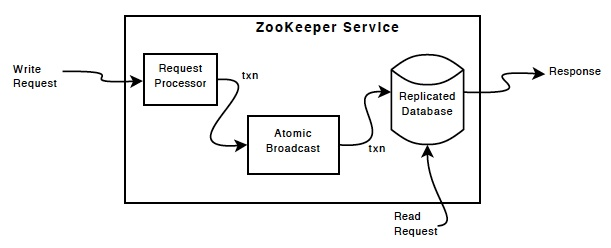
\includegraphics[width=0.8\textwidth]{images/zookeeper.jpg}
\centering
\caption{ZooKeeper Components}
%http://zookeeper.apache.org/doc/trunk/images/zkcomponents.jpg
\end{figure}

Every ZooKeeper server services clients and clients connect to exactly one server. To create a client session, the application code must provide a connection string containing a comma separated list of host:port pairs, each corresponding to a ZooKeeper server. The ZooKeeper client library will pick an arbitrary server and try to connect to it. If the client becomes disconnected from the server, the client will automatically try the next server in the list until a connection is re-established.

To provide high read throughput, ZooKeeper services the read requests from the local replica of state at each server. In contrast, all write requests are forwarded to a single server, referred as to the leader. The leader uses an atomic broadcast protocol, called Zab\index{Zab}, to keep all the servers in sync \cite{Reed:2008:STO}. Such a leader is elected through a leader election algorithm and synchronized with a quorum of other servers, called followers. By sending all updates through the leader, non-idempotent requests are transformed into idempotent transactions. To guarantee the correct transformation, ZooKeeper enforces that there is only one leader in Zab. And the Zab protocol meets the following requirements:
\begin{description}
\item[Reliable delivery] If a message, $m$, is delivered by one server, then it will be eventually delivered by all correct servers.
\item[Total order] If message $a$ is delivered before message $b$ by one server, then every server that delivers $a$ and $b$ delivers $a$ before $b$.
\item[Causal order] If message $a$ causally precedes message $b$ and both messages are delivered, then $a$ must be ordered before $b$.
\item[Prefix property] If $m$ is the last message delivered for a leader $L$, any message proposed before $m$ by $L$ must also be delivered.
\end{description}

Zab at a high level is a leader based protocol similar to Paxos\index{Paxos} \cite{Lamport:1998:PP}. Compared to Paxos, Zab is primarily designed for primary-backup systems rather than for state machine replication.
The Zab protocol consists of two modes: recovery/leader activation and broadcast/active messaging. When the service starts or after a leader failure, Zab transitions to recovery mode. Recovery mode ends when a leader emerges and a quorum of servers have synchronized their state with the leader. Synchronizing their state consists of guaranteeing that the leader and new server have the same state.
Once a leader has a quorum of synchronized followers, it accepts messages to propose and coordinates message delivery. The broadcast looks just like two-phase commit \cite{opac:2009} without the need to handle aborts and all communication channels are assumed FIFO:
\begin{itemize}
\item The leader sends proposals to all followers in the order that requests have been received. Before proposing a message the leader assigns a monotonically increasing unique zxid.
\item Followers process messages in the order they are received.
\item The leader will issue a COMMIT to all followers as soon as a quorum of followers have ACKed a message.
\item Followers deliver the message when they receive the COMMIT from the leader.
\end{itemize}

\section[HBase]
{HBase}
Apache HBase \cite{HBase}\index{HBase} is modeled after Google's BigTable \cite{Chang:2006:BDS}\index{BigTable}, implemented in Java, and run on top of Apache Hadoop. A competing open source project is Apache Accumulo \cite{Accumulo}\index{Accumulo} that shares very similar architecture and features (especially now HBase 0.98 supports cell-level security that was a unique offer from Accumulo).

\subsection{Data Model}

In BigTable-like stores, data are stored in tables, which are made of rows and columns. Columns are grouped into column families. A column name is made of its column family prefix and a qualifier. The column family prefix must be composed of printable characters. The column qualifiers can be made of any arbitrary bytes. In HBase, column families must be declared up front at schema definition time whereas new columns can be added to any column family without pre-announcing them. The only way to get a complete set of columns that exist for a column family is to scan all the rows.

Table row keys are uninterrpreted byte arrays. Rows are lexicographically sorted by row keys. In HBase, the empty byte array is used to denote both the start and end of a table's namespace.
A cell's content is an uninterpreted array of bytes. And table cells are versioned. A (row, column, version) tuple exactly specifies a cell. The version is specified using a long integer. Typically this long contains time instances.

The four primary data model operations are Scan, Get, Put, and Delete. Scan allows iteration over multiple rows while Get returns columns for a specified row. It can be specified to retrieve everything, or all columns from specific families, or specific columns.
By default, when doing a Get, the latest/highest version of the cell is returned. It is possible to return more than one version with Get.setMaxVersions() or to return versions other than the latest by Get.setTimeRange(). Without specifying the version, Put always creates a new version of a cell with the server's currentTimeMillis. But the user may specify the version on a per-column level. The user-provided version may be a time in the past or the future, or a non-time purpose long value. To overwrite an existing value, an exact version should be provided. Delete can happen on a specific version of a cell or all versions. To save space, HBase also cleans up old or expired versions. To declare how much data to retain, one may define the number of versions or the time to live (TTL).

Deletes work by creating tombstone markers. Once a tombstone\index{Tombstone} marker is set, the ``deleted'' cells become effectively invisible for Get and Scan operations but are not immediately removed from store files. There is a snag with the tombstone approach, namely ``Deletes mask Puts''\index{Deletes mask Puts}. Once a tombstone marker is set, even Puts after the Delete will be masked by the delete tombstone. Performing the Put will not fail. However when you do a Get, the Put has no effect but will start working  after the major compaction, which will really remove deletes and tombstone markers.

\subsection{Storage}

Physically, HBase uses HDFS to store data. Empty cells are not stored as tables usually have a large number of columns and are very sparse. In HBase, tables are stored on a per-column family basis. All column family members are stored together on HDFS. 
Recall that HDFS is a write-once (appending-only since 0.20) file system. It is very efficient for reading a large portion of  big files but not designed for random access. So how does HBase provide random, realtime read/write access on top HDFS (which is actually the exact reason to build HBase)? Here we come to the concept of Store. In HBase, a Store corresponds to a column family in a Region (see next section for details). A Store hosts a MemStore\index{HBase!MemStore} and a set of zero or more StoreFiles\index{HBase!StoreFile}. The MemStore holds in-memory modifications to the Store \footnote{In contrast, the BlockCache keeps data blocks resident in memory after they're read.}. When the MemStore reaches a certain size or the total size of all MemStores reaches the upper limit (both are configureable), the sorted key-value pairs (the key is a (row, column, version) tuple) in MemStore will be flushed into a HDFS file called StoreFile in HFile\index{HBase!HFile} format \footnote{Earlier versions used the MapFile\index{HDFS!MapFile} format. The MapFile is actually a directory that contains two SequenceFile: the data file and the index file. }.

HFile is based on SSTable\index{BigTable!SSTable} file in the BigTable. An SSTable provides a persistent, ordered immutable map from keys to values, where both keys and values are arbitrary byte strings. Because it is ordered, SSTable supports both lookups by key and iterations over all key-value pairs in a specified key range. Each SSTable contains a sequence of blocks of configurable size. The end of SSTable contains a location index of blocks. With the index loaded into memory, a lookup can be performed with a single disk seek. The appropriate block is found by a binary search in the in-memory index and is then read from disk. An SSTable may be completely mapped into memory to avoid frequent I/O operations.

For a valid write operation, it is firstly written to the write-ahead-log (WAL)\index{Write ahead log} and then its contents are inserted into the MemStore. In contrast, a read operation is performed on the merged view of the MemStore and all StoreFiles. If there are a lot of StoreFiles that are not in memory, a read operation will involve many disk accesses. To reduce the number of I/O, Bloom filters \cite{Bloom:1970:STH} can be created for StoreFiles of a particular Store (in HFile v2, Bloom filters are created at block level). By checking if a StoreFile might contain a specified key with Bloom filters, HBase significantly reduces the number of disk seeks required for read operations. Bloom filters also avoid disk access for most lookups of non-existent keys.

A Store may have many StoreFiles that are created for each flush. Over time, many versions of a row may exist in different StoreFiles. Each of these versions may have different sets of columns. Thus, reading a whole (or a large portion of) row could require many seeks in different files if too many files accumulate. In order to reduce the number of StoreFiles per Store, a background process called compaction is executed to merge StoreFiles. There are two types of compactions: minor and major. Minor compactions pick up a couple of smaller adjacent StoreFiles and rewrite them as one. Minor compactions do not drop deletes and expired cells. In contrast, major compactions pick up all the StoreFiles in the Store and generate a single StoreFile per Store that removes deletes and expired cells.

The compaction improves the average latency of reads at the expense of rewriting the same data multiple times (write amplification). Especially, the strategy how to choose files to merge in minor compaction has a big impact on the balance between read performance and write amplification. HBase supports pluggable compaction policies, including ratio based, exploring, and stripe compaction.

This storage design is actually a kind of log-structured merge-tree (LSM tree) \cite{O'Neil96thelog-structured}\index{LSM tree}, which maintains data in two (or more) separate structures, each of which is optimized for its respective underlying storage medium. And data is synchronized between the two structures efficiently. A log-structured storage engine avoids overwrites and uses sequential writes to update data, which is friendly for both hard disks (HDD) and solid-state disks (SSD). The sequential writes avoid random disk seek on HDD and thus greatly improve latency. On SSD, sequential writes avoids write amplification and disk failure and thus improve both performance and SSD lifetime. Besides HBase,  LevelDB, RocksDB, WiredTiger, Apache Cassandra, and SQLite4 also employ LSM trees.

\subsection{Architecture}

HBase is a distributed database designed to run on a cluster of machines. HBase supports horizontal scalability by auto-sharding, which means that tables are dynamically partitioned by rows and distributed by the system. 

\begin{figure}[t]
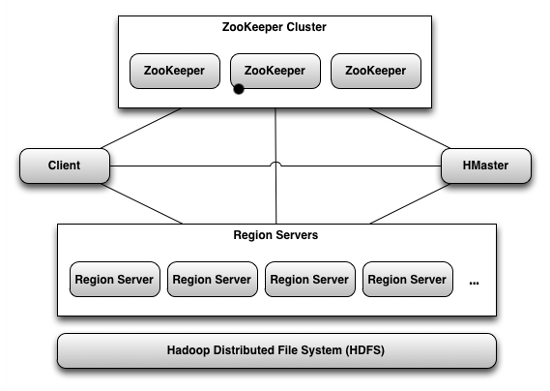
\includegraphics[width=0.8\textwidth]{images/hbase-architecture.png}
\centering
\caption{HBase Architecture}
%https://i0.wp.com/dgdsbygo8mp3h.cloudfront.net/sites/default/files/Article-Images/7140_08_01.png
\end{figure}

\subsubsection{Sharding}

The basic unit of sharding is called a Region\index{HBase!Region} in HBase. A region is a contiguous and sorted range of rows of a table stored together on disk. Initially, there is only one region for a table. However, when regions become too large, a region is split into two at the middle key (recall that rows are lexicographically sorted by row keys). Regions are served by RegionServer\index{HBase!RegionServer}. Each RegionServer is responsible a set of regions but one region can be served only by one RegionServer.

Typically, HBase setups a RegionServer co-located with an HDFS DataNode on the same physical node. When StoreFiles are written into HDFS, one copy is written locally and two are written to other nodes. As long as the regions are not moved, there is good data locality. When the regions are reassigned to a new RegionServer, the data locality is lost and the RegionServer needs to read the data over the network from remote DataNodes until the data is rewritten locally.

In general, HBase is designed to run with a small (20-200) number of relatively large (5-20Gb) regions per RegionServer. A large number of regions per RegionServer will cause a lot memory overhead and possibly too many flushes and compactions. When there are too many regions, one can consolidate them with the utility Merge.

The coordination work of assigning a region to a RegionServer is done by the Master server, which is implemented by HMaster\index{HBase!HMaster}. The Master typically runs on the NameNode. Each region is assigned to a RegionServer on startup. However, the Master may decide to move a region from one RegionServer to another for load balance. Besides, the Master also handles RegionServer failures by assigning the regions to another RegionServer.  The Master also performs administrative operations such as monitoring all RegionServer instances and all metadata changes (e.g. create, modify, and delete tables or column families).

The catalog table hbase:meta (previously called META), maintained by the Master, keeps a list of all regions in the system. The hbase:meta exists as an HBase table. However, it cannot be split and therefore consists of a single region. The location of hbase:meta is stored in Zookeeper. For each region, the hbase:meta table contains the region id, table name, start key, the RegionServer serving this region, etc.

The HBase client consists of two main parts: HBaseAdmin\index{HBase!HBaseAdmin} and HTable\index{HBase!HTable}. HBaseAdmin communicates with the Master to execute administrative operations. HTable communicates directly with the RegionServers to manipulate data. To locate the RegionServers that are serving the particular row range of interest, HTable queries the hbase:meta table. It then contacts the corresponding RegionServer directly for data access. The region information is cached in the client so that subsequent requests need not go through the lookup process. If a region be reassigned, the client will refresh the location information by querying hbase:meta.

\subsubsection{Fault Tolerance}

The Master looks like a single point of failure. Actually, we can set up multiple Masters although only one is active. If the active Master shuts down or loses its lease in ZooKeeper, the remaining Masters compete to take over the active role. Because the clients talk directly to the RegionServers, the HBase cluster can still function in a steady state in short period during the Master failover.

Recall that a region is managed by a single RegionServer at a time. If a RegionServer fails, the corresponding regions are not available until the detection and recovery steps have happened. It is actually a single point of failure although there are no global failures in HBase. Especially when the RegionServer serving hbase:meta fails, the Master cannot perform administrative tasks and new clients cannot proceed as normal.

To be resilient to node failures, all StoreFiles are written into HDFS. Besides, the write-ahead-log (WAL)\index{Write ahead log} is also written into HDFS. The Master detects the silent death of RegionServers by watching the connections between RegionServers and ZooKeeper. ZooKeeper itself employs heartbeats. On a timeout, the Master declares the RegionServer as dead and starts the recovery process. During the recovery, the regions are reassigned to random RegionServers and each RegionServer reads the WAL to recover the correct region state. This is a complicated process and the mean time to recovery (MTTR\index{MTTR}) of HBase is often around 10 minutes if a DataNode crash with default settings. But we may reduce the MTTR to less than 2 minutes with careful settings \cite{HBaseMTTR}.

\subsubsection{Cluster Replication}

HBase provides a cluster replication mechanism which keeps one cluster's state synchronized with that of another cluster. Cluster replication is useful to backup and disaster recovery, geographic data distribution, or offline data analytics, etc. Cluster replication employs a source-push methodology that uses the WAL of the source cluster to propagate the changes. The WAL records all the mutations (Put/Delete) and the source cluster Region Servers ship the edits to the destination cluster Region Servers, which replay all the updates. The replication is done asynchronously and each RegionServer replicates their own stream of WAL edits. In a write heavy application, the destination cluster may notably lag behind from the source. Zookeeper plays a key role in cluster replication, where it coordinates almost all the major replication activities.

In practice, cluster replication can be implemented in multiple modes:
\begin{description}
\item[Master-Slave Replication]
The replication is done in a single direction, i.e., transactions from one cluster are pushed to other cluster.
\item[Master-Master Replication]
The replication is sent across in both the directions, for different or same tables, i.e., both the clusters are acting both as master and slave. In the case that they are replicating the same table, cluster id is used to prevent replication loops.
\item[Cyclic Replication]
More than two clusters takes part in replication setup. There are various possible combinations of master-slave and master-master set up between any two clusters. 
\end{description}

\subsubsection{Consistency}
Because one region can be served only by one RegionServer, HBase provides row level consistency. In fact, HBase supports row-level ACID\index{ACID} in limited ways. Basically, multiple Puts and Deletes to the same row provide all ACID guarantees. Besides, the \texttt{mutateRowsWithLocks} method of \texttt{HRegion} can be used by coprocessors to implement atomic operations at the region level.

But HBase does not guarantee any consistency between regions. Although all rows returned will consist of a complete row that existed at some point in the table's history, a Scan is not a consistent view of a table. Moreover,  HBase has no mixed read/write transactions.

\subsubsection{Timeline-Consistent High Available Reads}
With the design that each region is served by only one RegionServer, HBase has the strong consistency guarantee. However, when a RegionServer become unavailable, the hosted regions become unavailable during detection and recovery. On the other hand, some applications prefer high availability for reads. For example, the data may be read-only or stale data is acceptable. Through ``region replication'', HBase provides timeline-consistent high available reads. In this mode (region replication is set to 2 or more), the master will assign the replicas of the regions to multiple RegionServers.  All of the replicas for a single region will have a unique replica\_id, starting from 0. The region replica having replica\_id 0 is called the primary region, and the others secondary regions. Only the primary can accept writes from the client and thus the writes are not highly-available. The writes are asynchronously sent to the secondary region replicas using Async WAL replication, which works similarly to cluster replication but instead happens inside the cluster.

For reads, one may provide an additional consistency parameter (STRONG or TIMELINE). In case of the STRONG consistency, the read is always performed by the primary regions. In case of TIMELINE consistency, the read RPC will be sent to the primary region server first. If the primary does not respond back in a short interval (10ms by default), parallel RPC to secondary region replicas will be sent. Then the result is returned from whichever RPC is finished first. The API Result.isStale() is added to inspect if the result is from a secondary region.

The feature is called timeline-consistent because the secondaries apply the edits in the order that the primary committed them. Therefore, the secondaries will contain a snapshot of the primaries data at any time point. However, the client could observe edits out-of-order, and can go back in time, if it observes reads from one secondary replica first, then another secondary replica because there is no stickiness to region replicas or a transaction-id based guarantee.

Note that the goal and design of this feature is not to balance the load of reads because the read requests are always sent to the primary. Instead, it tries to satisfy the low latency guarantees for some applications.

\subsection{Security}
Data security is important for any real world applications. HBase offers a strong security model including authentication, authorization, and encryption.

HBase can be configured to use Kerberos\index{Kerberos} authentication at the RPC layer via Simple Authentication and Security Layer (SASL)\index{SASL}. If enabled, it ensures that only authorized users can communicate with HBase. Note that the underlying HDFS should also be configured to use strong authentication. Otherwise, there is no benefit at all. Even better, HBase optionally supports transparent encryption for protecting HFile and WAL data at rest. Besides, the RPC between HBase and clients can also be configured to employ encrypted communication.

Once the users are authenticated via Kerberos, HBase's authorization mechanism allows restricted access for specified users.
An access control list (ACL) specifies which users shall be granted access to an object (table or column family), as well as which operations (read, write, create, execute, admin) are allowed. Note that the hbase:meta table is readable by every user, regardless of the user's other grants or restrictions.

\subsubsection{Cell Level Security}

Since version 0.98, ACLs in HBase can be specified at the cell scope. Cell-level ACLs are implemented using tags, which require HFile v3. A tag is a piece of metadata which is part of a cell, separate from the key, value, and version.  Besides cell-level ACLs,  HBase can store visibility expressions into tags, providing cell-level security capabilities similar to Apache Accumulo. The visibility labels allow us to label cells and control access to labelled cells, to further restrict who can read or write to certain subsets of the data. 

When mutations are applied, users can specify a security label for each cell by passing a CellVisibility object. Security labels consist of a set of user-defined tokens that are required to read the associated cell. The security label expression syntax supports boolean logic operations. When a client attempts to read data, any security labels present are examined against the set of authorizations passed with Scanner. If the authorizations are determined to be insufficient to satisfy the security label, the cell is suppressed from the results. Each user has a set of associated security labels, which can be manipulated in the shell.

Both ACL controller and visibility label controller are implemented as coprocessors, which we will discuss in details in what follows.

\subsection{Coprocessor}

Coprocessors\index{HBase!Coprocessor} provide a powerful way to add custom functionalities at the server side against locally-stored data \cite{HBaseCoprocessor}. This allows users to efficiently summarize, filter, and aggregate data directly on RegionServers. Compared to MapReduce, it gives a dramatic performance improvement by removing communication overheads. 

The HBase coprocessor framework provides a library and runtime environment for executing user code within the RegionServers and the Master process. Coprocessors that can be loaded globally on all tables and regions hosted by a region server are called system coprocessors. In contrast, coprocessors that are loaded on all regions for a table on a per-table basis are known as table coprocessors. Moreover, the framework supports two different types of coprocessors, the observers and the endpoints.

The observers, like triggers in RDBMS, are executed from core HBase code when certain events occur. HBase includes three observer interfaces: RegionObserver provides hooks for data manipulation events; WALObserver provides hooks for write-ahead log related operations; and MasterObserver provides hooks for DDL-type operation. Multiple observers can be loaded at one place and they are chained to execute sequentially by order of assigned priorities.

The endpoints, resembling stored procedures, can be invoked at any time from the client and be executed remotely at the target region or regions. The endpoint is an interface for dynamic RPC extension. The endpoint implementation is installed on the server side and can then be invoked with HBase RPC. The client library provides convenience methods for invoking such dynamic interfaces.

\subsection{Summary}
As a BigTable clone, HBase provides a wide-column data model and random real-time CRUD operations on top of HDFS. They can horizontally scale out to efficiently serve billions of rows and millions of columns by auto-sharding. Because each region is served by only one RegionServer at a time, they also support strong consistency for reads and writes. Automatic failover of RegionServer is supported although efforts are needed to reduce MTTR. With replications across multi data centers, HBase adds more supports of disaster recovery.

\section[Riak]
{Riak}
Riak \cite{Riak}\index{Riak} is a highly available key-value store from Basho Technologies. Riak is written in Erlang and is modeled after Amazon.com's Dynamo \cite{DeCandia:2007:DAH}\index{Dynamo}. It is designed to provide an ``always-on'' experience while sacrificing consistency under certain scenarios. Riak is architected for low-latency, high availability, fault-tolerance, operational simplicity, and scalability.

\subsection{Data Model}

Riak has a schemaless design and organizes data into the Buckets of Objects. A buckets is essentially a flat namespace and an object is comprised of a key/value pair. The unique keys in a bucket are simply opaque binary strings to identify objects. Interaction with the database is by retrieving or modifying the entire object/value. There is no partial fetch or update of the data. Besides, no operations (Get, Put, Post, and Delete) span multiple data items.

Although it is very simple, the key/value pair data model is very flexible. For example, it is frequently used for session storage, user accounts, settings, and preferences, etc. In general, the applications should be able to get the keys ``for free'', without having to perform any queries to discover them, e.g. user id, session id, etc. If Bitcask is used as storage backend, Riak also supports automatic expiry of keys, which is helpful to session management \footnote{Riak was originally created to serve as a highly scalable session store.}. Since it is schemaless, binaries such as images and PDF documents can be stored directly \footnote{It is not recommended to store objects over 50M for performance reasons.}. On the other hand, structured data (e.g. relational tables) should be denormalized and usually stored as JSON or XML.

Initially, Riak is completely agnostic toward the data stored within it. However, Riak introduces several eventually convergent Data Types in version 2.0. Inspired by \cite{CRDT2011}, Riak Data Types are convergent replicated data types (CRDTs\index{CRDT}, also called commutative replicated data types). By default, Riak is an eventual consistency system, in which a replica may execute an operation without synchronizing with other replicas. The operation is sent asynchronously to other replicas; every replica eventually applies all updates, possibly in different orders. Conflict resolution can be very difficult in Riak, which we will discuss in details later.

Riak Data Types are introduced to relieve developers on conflict resolution in some situations with builtin convergence logic. Riak currently provides five CRDTs: \texttt{flag}, \texttt{register}, \texttt{counter}, \texttt{set}, and \texttt{map}. They are operations based from the point view of Riak clients. Of them, flags and registers cannot be stored in a bucket/key by themselves. Instead, they must be embedded in \texttt{map}s.

\begin{description}
\item[Flag]
A flag may take the value \texttt{enable} or \texttt{disable}.
Flags support only two operations: \texttt{enable} and \texttt{disable}.

\item[Register]
Registers are essentially named binaries.
The only operation that registers support is to change the binaries stored in them.

\item[Counters]
Counters take integer values and support increment and decrement operations. Therefore, it is not necessary to fetch, mutate, or put a counter.

\item[Sets]
Sets are collections of unique binary values.
The available operations on sets include add an element, remove an element, add multiple elements, or remove multiple elements.

\item[Maps]
A map is a collection of fields that supports the nesting of multiple Data Types, including maps themselves. One can add or remove fields to/from the map.
\end{description}

In the section of Consistency, we will discuss the details how Data Types resolve conflicts.

\subsection{Storage}

In contrast to HBase and Accumulo replying on complicated Hadoop HDFS, Riak stores data in the native file system. Moreover, Riak supports pluggable storage backends, including Bitcask, LevelDB, and Memory. It is possible to run multiple backends within a single Riak cluster, which employs different storage backends for different buckets. 

\subsubsection{Bitcask}
Bitcask is the default storage backend and uses a log-structured hash table design \cite{Bitcask}\index{Riak!Bitcask}. A Bitcask instance is a directory, and only one process can open the Bitcask for writing at a given time. At any time point, the file being written is called the active file of Bitcask. When the active file meets a size threshold it will be closed and a new active file will be created. Once a file is closed, it is considered immutable and will never be opened for writing again. The active file is only written by appending a key/value entry (with timestamp and crc). Deletion is simply a write of a special tombstone value. Thus, a Bitcask data file is simply a linear sequence of the key/value entries. Such a log structured design allows for minimal disk head movement for a stream of writes.

Bitcask keeps an in-memory hash-table of all keys, called keydir. A keydir maps every key in a Bitcask to a data structure including file id, value size, value position in the file, and timestamp. After an append completes, keydir is updated too.
With the kydir, a read needs only single disk seek. However, it also results in a memory-bounded keyspace.

A Bitcask may use up a lot of space over time because old or deleted values still exist in the files. A merge process is used for the compaction of Bitcask. The merge process iterates over all non-active files in a Bitcask and produces a set of data files containing only the live or latest versions of each present key. Besides, it also creates a hint file for each data file. A hint file is like the data files but each entry contains the position and size of the value instead of the value itself.

During the startup, we scan all of the data files in a Bitcask to build the keydir. If the hint file exists for a data file, it will be scanned instead for a much quicker startup time.

\subsubsection{LevelDB}
To store a large number of keys, LevelDB is preferred. LevelDB\index{LevelDB} is an open source on-disk key-value store \cite{LevelDB}\index{LevelDB}. It shares the same general design as the BigTable tablet stack and is written by Google fellows Jeffrey Dean and Sanjay Ghemawat. LevelDB supports batching writes, forward and backward iteration, and compression of the data via Google's Snappy compression library.

Although LevelDB uses a similar MemTable/SSTable design as BigTable, the organization of the database files is different. Each database is represented by a set of files organized into a sequence of levels. Each level stores approximately ten times as much data as the previous level. Especially, an appending-only log file stores a sequence of recent updates. When the log file reaches a pre-determined size, it is converted to a sorted table and a new log file is created for future updates. The sorted table generated from a log file is placed in a special {\em young} level (also called level-0).

Within a level ($L > =1$), LevelDB guarantees there's no overlapping in SSTables, meaning a row can appear at most in one file on a single level. When the size of level $L$ exceeds its limit (says $10^L$ MB), LevelDB will compact it in a background thread. The compaction picks a file from level $L$ and all overlapping files from the next level $L+1$. A compaction merges the contents of the picked files to produce a sequence of level-($L+1$) files. During compaction, LevelDB will create a new level-($L+1$) file when the current output file has reached the target file size, or the key range of the current output file has grown enough to overlap more then ten level-($L+2$) files. The second rule ensures that a later compaction of a level-($L+1$) file will not pick up too much data from level-($L+2$). Compactions for a particular level rotate through the key space. 

Compactions from level-0 to level-1 are treated specially because files in level-0 may overlap each other. When the number of young files exceeds a certain threshold, all of the young files are merged together with all of the overlapping level-1 files to produce a sequence of new level-1 files. The compactions gradually migrate new updates from the young level to the largest level. There is no major compaction that merge all files into one.

LevelDB may have to do a few disk seeks to satisfy a read: one disk seek per level. The worst case is bounded at the total number of levels. But it may require much less disk seek in practice. If 10\% of the database fits in memory, only one seek for the last level is needed because all of the earlier levels should end up cached in the OS buffer cache for most file systems. If 1\% fits in memory, LevelDB will need two seeks.

Riak uses a fork of LevelDB, which is optimized to meet Basho's requirements such as multiple databases running simultaneously, fast disaster recovery, aggressive delete logic, etc. For example, this fork moves away from the original single thread design to a thread pool that can run simultaneous companions on the same database as well as other databases.

\subsubsection{Memory}
The Memory\index{Riak!Memory} storage backend uses in-memory tables to store all data (both keys and values) but the data is never saved to disk or any other persistence storage. It may be useful to store small amounts of transient state.

\subsection{Architecture}

\begin{figure}[t]
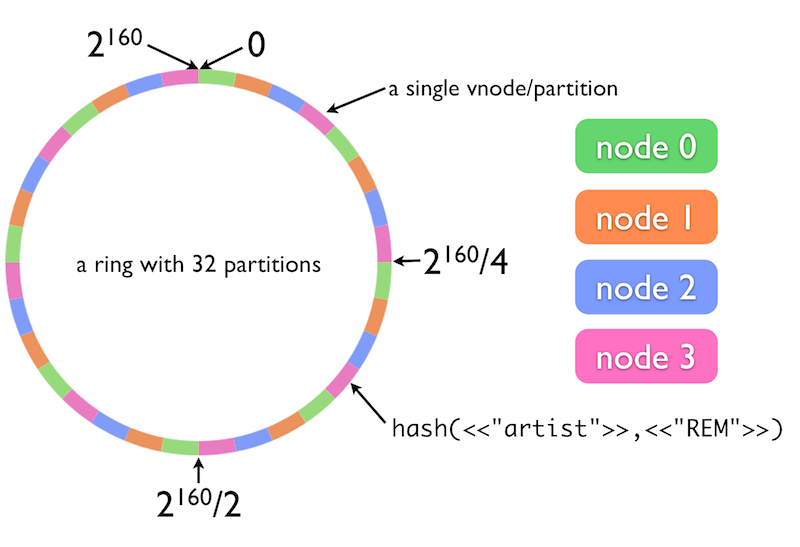
\includegraphics[width=0.8\textwidth]{images/riak-ring.png}
\centering
\caption{Riak Ring}
%https://i0.wp.com/docs.basho.com/shared/1.1.4/images/riak-ring.png?1372706703
\end{figure}

All nodes in a Riak cluster are equal. Each node is fully capable of serving any client request. There is no ``master''. This uniformity provides the basis for Riak's fault-tolerance and scalability. The symmetric architecture is based on consistent hashing to distribute data around the cluster. In consistent hashing, the output range of a hash function is treated as a ring. Riak uses the SHA1 hash function to map the keys of data items to an 160-bit integer space which is divided into equally-sized partitions. Each virtual node (vnode) will claim a partition on the ring. The physical nodes each attempt to run roughly an equal number of vnodes. Consistent hashing ensures data is evenly distributed around the cluster.

Nodes can be added and removed from the cluster dynamically and Riak will redistribute the data accordingly. The ring state is shared around the cluster by a gossip protocol. Whenever a node changes its claim on the ring, it announces its change via this protocol. It also periodically re-announces what it knows about the ring, in case any nodes missed previous updates.

Riak automatically and asynchronously replicates data to $N$ (default $N=3$) separate partitions on the Riak Ring. Note that $N=3$ simply means that three different partitions/vnodes will receive copies of the data. There are no guarantees that the three replicas will go to three different physical nodes although Riak attempts to distribute the data evenly.

\begin{figure}[t]
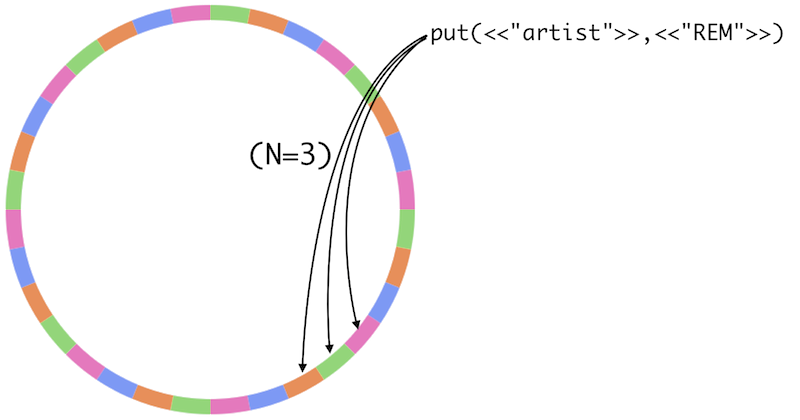
\includegraphics[width=0.8\textwidth]{images/riak-data-distribution.png}
\centering
\caption{Riak Data Distribution}
%https://i0.wp.com/docs.basho.com/shared/1.1.4/images/riak-ring.png?1372706703
\end{figure}

For a write/Put request, any node may participate as the coordinator for the request. The coordinating node consults the ring state to determine which vnode owns the partition which the value's key belongs to, then sends the Put request to that vnode, as well as the vnodes responsible for the next $N-1$ partitions in the ring. The Put request may also specify that at least $W$ ($<= N$) of those vnodes reply with success, and that $DW$ ($<= W$) reply with success only after durably storing the value. 

The read/Get request operates similarly. The request is sent to the vnode/partition in which the key resides, as well as to the next $N-1$ partitions. The request also specifies $R$ ($<= N$), the number of vnodes that must reply before a response is returned. With $R=1$, the client will get faster response but take a chance of receiving an old copy.

To ensure high variability during node failures and network partitions, Riak uses the concept of ``sloppy quorum''\index{Riak!Sloppy quorum}. That is, all read and write operations are performed on the first $N$ healthy nodes from the preference list, which may not always be the first $N$ nodes encountered while walking the consistent hashing ring.
When a node is unavailable, the neighboring nodes will temporarily accept its write requests \footnote{The first reads will return the error 404 Not Found.}. When the node returns, data is transferred to the primary node via the ``hinted handoff''\index{Riak!Hinted Handoff} process.

\subsection{Consistency}
By default, Riak is an eventual consistency system, in which a replica may execute an operation without synchronizing with other replicas. Therefore, conflicts between replicas of an object are inevitable.

In read and write requests, the default values of $R$ and $W$ are quorum, where quorum indicates a majority of the $N$ value ($N/2+1$, or 2 for the default $N$ value of 3). Consider that a failed node just recovered but does not have requested key-value or has an old copy, or that the client reads the value immediately after a successful write such that the replication process is not finished yet. Because $W=2$ and $R=2$, the coordinating node will receive at least one response with latest value, which will be returned to the client. In general, one should set $W+R>N$ so that a read hopefully reflects the most recent write.
Meanwhile a read repair process will occur to force the errant nodes to update their object values based on the value of the successful read. 
Read repair is a passive process that is only triggered when data is read. Riak also has an automatic background process called active anti-entropy (AAE) that compares and repairs any divergent, missing, or corrupted replicas.

In above, we simply say that the read returns ``latest'' value with $W+R>N$. However, it sounds simple but is actually very challenging to determine which copy is newer.

\subsubsection{Last Write Wins}
A simple strategy is last-write-wins (LWW)\index{Last-write-wins}, which is based on timestamps (recall that Riak attaches a timestamp for each write). On a single server, we can easily to tell which write is newer based on timestamp regardless of the accuracy of system clock (assuming that the clock is always increasing). However, the definition of ``last'' is hard in a distributed system as clocks can not be perfectly synchronized.
Therefore, last-write-wins will necessarily drop some acknowledged writes in the case of concurrent updates. A more reliable way to use logical time such as vector clock or dotted version vector.

\subsubsection{Vector Clock and Dotted Version Vector}
When a value is stored in Riak, it is tagged with a piece of metadata called a ``causal context''\index{Riak!Causal context} which establishes the object's initial version. Causal context comes in one of two possible forms: vector clock and dotted version vector.

Vector clock \cite{fidge1988timestamps, Mattern89virtualtime}\index{Vector clock} is an algorithm for generating a partial ordering of events in a distributed system and detecting causality violations. A vector clock of a system of $N$ processes is a vector of $N$ logical clocks, one clock per process. When a key-value pair is added into bucket, it is tagged with a vector clock of all zeros as the initial version. Later the vector clock is extended for each update so that two versioned replicas can be compared to determine:
\begin{itemize}
\item Whether one object is a direct descendant of the other
\item Whether the objects are direct descendants of a common parent
\item Whether the objects are unrelated in recent heritage
\end{itemize}

Vector clocks can detect concurrent updates to the same object but they may have the problem ``sibling explosion''. If an object is updated by five different clients concurrently and tagged with the same vector clock, then five values should be created as siblings. Depending on the order of delivery of those updates to the different replicas, however, sibling values may be duplicated and then result in sibling explosion.

Dotted version vector \cite{Preguica:2012:BAE}\index{Dotted version vector}, on the other hand, identify each value with the update that created it. If five clients concurrently update the object, each of these updates will be marked with a dot (a minimal vector clock) that indicates the specific event that introduced it. Therefore, duplicate values can be identified and removed, reducing the likelihood of sibling explosion

With causal context, each node of replicas can auto-repair out-of-sync data when feasible. For siblings that are created by multiple clients that concurrently reads a key-value and writes it back, Riak cannot reconcile automatically. Prior to version 2.0, Riak simply accepts both writes. When a read comes for the same key, Riak sends all the versions for that key and lets the client to do manual reconciliation.

To relieve developers from handling data convergence at the application level, Riak introduces Data Types, which have builtin convergence rules: 

\begin{center}
\begin{tabular}{ l p{3in} }
\hline
\textbf{Data Type} & \textbf{Convergence rule} \\
\hline
Flags	& \texttt{enable} wins over \texttt{disable}. \\
Registers	& The most chronologically recent value wins, based on timestamps. \\
Counters	& Each actor keeps an independent count for increments and decrements; upon merge, the pairwise maximum of the counts for each actor will win. \\
Sets	        & If an element is concurrently added and removed, the add will win. \\
Maps       & If a field is concurrently added or updated and removed, the add/update will win. \\
\hline
\end{tabular}
\end{center}

Note that Riak Data Types do not guarantee strong consistency. Besides, the built in convergence rules may not be suitable in your applications. 

\subsubsection{Strong Consistency}
In version 2.0, strong consistency was added to complement Riak's standard eventually consistent, high availability mode. When data is stored in a bucket with strong consistency guarantees, a value is guaranteed readable by any client immediately after a successful write has occurred to a given key. In this sense, single-key strongly consistent operations are atomic, and operations on a given key are linearizable. In this mode, a quorum of primary vnodes responsible for the key must be online and reachable or the request will fail.

\subsection{Summary}
In the default mode, Riak is in the school of AP systems to provide an ``always-on'' experience. With a symmetric design, all nodes in a Riak cluster are equal and each node is fully capable of serving any client request. With sloppy quorum and hinted handoff, Riak can process client requests even during node failures or network partitions. On the other hand, the eventually consistent model also bring a lot of challenges to developers. Riak provides multiple options such as last-write-wins, causal context, and Data Types to help conflict resolution. They are suitable for different use cases although none provides strong consistency. Finally, Riak 2.0 has an optional mode to guarantee strong consistency. It is the user's call to be AP or CP.

\section[Cassandra]
{Cassandra}
Apache Cassandra \cite{Lakshman:2010:CDS, Cassandra}\index{Cassandra} is a hybrid of BigTable's data model and Dynamo's system design. Therefore, Cassandra provides the flexible wide columnar model, and has linear scalability and proven fault-tolerance on commodity hardware. Besides, Cassandra's support for replicating across multiple data centers is best-in-class. Since many features of Cassandra are already covered in previous sections as they are shared with HBase and Riak, we will focus on the additional unique features in what follows.

\subsection{Data Model}

Cassandra provides a two-dimensional row-column view to the data contained in a keyspace (i.e. table in HBase). Keyspaces are used to group column families together. If you need higher dimension to organize application data, there is the concept of super columns, which are columns that contain columns. However, super column is deprecated because of performance issues. Instead, developers are encouraged to use composite columns that was introduced in version 0.8.1. 

Before jumping into composite columns, we need to understand column sorting. Just like other key-value pair databases, the data type of keys and values in Cassandra are byte arrays. More interestingly, we can specify how column names will be compared for sort order when results are returned to the client. But why would we want to sort column names? This especially sounds strange to a relational database developer. In a relational database, we usually have tall tables, i.e. millions skinny rows with a handful columns. We could still follow this design in Cassandra although different rows do not have to share same column set. On the other hand, one wide row could have millions columns in BigTable-like database, actually up to 2 billion columns in Cassandra. In this case, column names are usually part of the data, rather than purely schema. For example, we can build inverted index with terms as the keys, document ids as the column names, and frequency as the value. One may even go with valueless columns, i.e. column names are data themselves and the values are not really meaningful. With wide-row design, it is necessary to compare column names sometimes, for instance, each row is the time series of stock price in a day and the column names are time points. You can use \texttt{compare\_with} attribute on a column family to tell Cassandra how to sort the columns. The default is \texttt{BytesType}, which is a straightforward lexical comparison of the bytes in each column. Other options are \texttt{AsciiType}, \texttt{UTF8Type}, \texttt{LexicalUUIDType}, \texttt{TimeUUIDType}, and \texttt{LongType}. You can also specify the fully-qualified class name to a class extending \texttt{org.apache.cassandra.db.marshal.AbstractType}. Again, we are sorting column names, not values. However, sorting column name providing a way to build second index, which is very useful in real world. Now come back to composite columns, which are arbitrary dimensional column names that can have types like CompositeType(UTF8Type, ReversedType(TimeUUIDType), LongType)). It is also really simple: it is implemented as a comparator so adds very little complexity.

\subsection{Storage}

Cassandra uses a storage structure similar to BigTable, including SSTable and MemTable. The details can be found in the section of HBase. Compared to HBase, Cassandra stores data in the native file system as Cassandra emphasizes operational simplicity.

\subsection{Architecture}

Same as Riak, Cassandra employs a ring topology but with more partition options. You can provide any IPartitioner\index{Cassandra!Partitioner} implementation to distribute data on nodes. Out of the box, Cassandra provides Murmur3Partitioner, RandomPartitioner, ByteOrderedPartitioner, and OrderPreservingPartitioner. Both Murmur3Partitioner and RandomPartitioner  force equal spacing of tokens around the hash space. ByteOrderedPartitioner orders rows lexically by key bytes. OrderPreservingPartitioner is similar to ByteOrderedPartitioner but treats keys as UTF8 strings. With OrderPreservingPartitioner the keys themselves are used to place on the ring. It brings data locality but also potential bottleneck on hot spots.

Beyond partitions, Cassandra also supports pluggable replication\index{Cassandra!Replication} strategies through IReplicaPlacementStrategy to ensure reliability and fault tolerance. Out of the box, Cassandra provides SimpleStrategy (rack unaware), LocalStrategy (rack aware) and NetworkTopologyStrategy (datacenter aware). In addition to setting the number of replicas, the strategy sets the distribution of the replicas across the nodes in the cluster depending on the cluster's topology. We are particularly interested in NetworkTopologyStrategy. With it, we can deploy the cluster across multiple data centers and specify how many replicas we want in each data center. If configured properly, Cassandra is able to read locally without incurring cross-datacenter latency, and handles failures nicely.

With NetworkTopologyStrategy, the first replica is placed according to the partitioner.
Additional replicas are placed by walking the ring clockwise until a node in a different rack is found. If no such node exists, additional replicas are placed in different nodes in the same rack.
To achieve this, we need a snitch maps IPs to racks and data centers. It defines how the nodes are grouped together within the overall network topology.

\subsection{CQL}
Initially, Cassandra provides a low level Thrift based API (insert, get, delete), similar to those of HBase. Later Cassandra introduces the SQL-like Cassandra Query Language (CQL\index{Cassandra!CQL}) as the best-practice interface. With CQL, schema is reintroduced and is conventional in most applications. Besides ease of use, native CQL drivers offering improved performance by providing connection pooling, failover, tracing support, etc.

The old wide columnar data model is still the foundation of Cassandra but CQL adds an abstraction layer that hides implementation details. In CQL, the data model is a partitioned row store, where rows are organized into tables and the first component of a table's primary key is the partition key. Within a partition, rows are clustered by the remaining columns of the compound primary key (called clustering columns).

Note that CQL does not bring the relational data model to Cassandra. For example, it does not support joins or subqueries. Rather, Cassandra emphasizes denormalization through collection types (set, list, and map)\index{Cassandra!Collection}.

CQL also provides secondary index to access data using attributes other than the partition key. It indexes column values in a separate, hidden table from the one that contains the values being indexed. The index is basically an inverted file. It is not suitable for high-cardinality columns, frequently updated or deleted columns, or searching for a row in a large partition unless narrowly queried.

\subsection{Consistency}

Like Riak, Cassandra also has read repairs and active anti-entropy to resolve some consistency issues. However, Cassandra's conflict resolution simply relays on last-write-wins. Cassandra 2.0 introduces ``compare and set'' based on Paxos consensus protocol, but misleadingly labels it as ``lightweight transaction''\index{Cassandra!Lightweight transaction}. A new IF clause has been introduced for both the INSERT and UPDATE commands that lets the user invoke lightweight transactions.

\subsection{Summary}
Overall, Cassandra is a very nice system with flexible data model, linear scalability and high availability. 
Cassandra offers robust support for clusters spanning multiple data centers. CQL provides a SQL-like alternative to the traditional RPC interface.
Apache Cassandra emphasizes operational simplicity. It does not require ZooKeeper or any other third-party components. It is very easy to configure and run. Actually Cassandra starts only one JVM per node, which brings a lot of simplicity to operation and maintenance.

\section[MongoDB]
{MongoDB}
Although key-value pairs are very flexible, it is tedious to map them to objects in applications. In this section, we will learn about a popular document-oriented database MongoDB \cite{MongoDB}\index{MongoDB}. MongoDB uses JSON-like documents with dynamic schemas, making the integration of data in certain types of applications easier and faster. Beyond key search, MongoDB supports search by value, range queries, and text searches. Any field in a document can be indexed (by B-Trees, similar to those in RDBMS).

\subsection{Data Model}

Documents are addressed in the database via a unique key. The documents contain one or more fields, and each field contains a value of a specific data type (maybe object or array). Documents that tend to share a similar structure are organized as collections. Compared to relational databases, collections could be considered analogous to tables and documents analogous to records. However, every record in a table has the same sequence of fields, while documents in a collection may have fields that are completely different. MongoDB stores documents in a binary representation called BSON (Binary JSON) \cite{BSON}\index{MongoDB!BSON}. The BSON encoding extends the JSON to include additional types such as date, int, long, double, byte array, etc.

\subsection{Storage}
MongoDB historically uses the memory mapped files for on-disk storage. From version 3.0, MongoDB supports pluggable storage engines, which means a rigorously defined interface between the database and the way it stores data. The pluggable storage engine API allows third parties to develop storage engines. In version 3.0, the additional storage backends include WiredTiger.

\subsubsection{Memory-Mapped Storage Engine}
With the memory-mapped storage engine (referred as to MMAPv1\index{MongoDB!MMAPv1}), MongoDB uses memory mapped files for managing and interacting with all data. A memory-mapped file is a segment of virtual memory which has been assigned a direct byte-for-byte correlation with some portion of a file or file-like resource. Once mapped, the relationship between file and memory allows MongoDB to interact with the data in the file as if it were memory.
MongoDB reads/writes to RAM directly and OS takes care of the rest. This greatly simplifies the cache and file access logic in MongoDB and also leverages OS's LRU (least recently used) cache behavior. On the other hand, it incurs the fragmentation management and read-ahead overhead. Clearly, this also limits the data size MongoDB can handle on 32-bit systems due to inherent memory limitations.

In this design, each database has a namespace file holding entries which each points to (the first extent of) a collection or index in data files. Data files are broken into contiguous disk space called extents (grow exponentially up to 2GB) to hold documents or B-Tree index nodes. Data files (and journals) are aggressively pre-allocated. MongoDB stores each document (plus some extra padding bytes as growth buffer) in an extent as a contiguous block. The documents are updated in-place and the whole document will be moved to a bigger space if the update increases the size of document beyond its current allocated space. All data files are memory mapped into the virtual memory of mongod, the primary daemon process for the MongoDB system.

\begin{figure}[t]
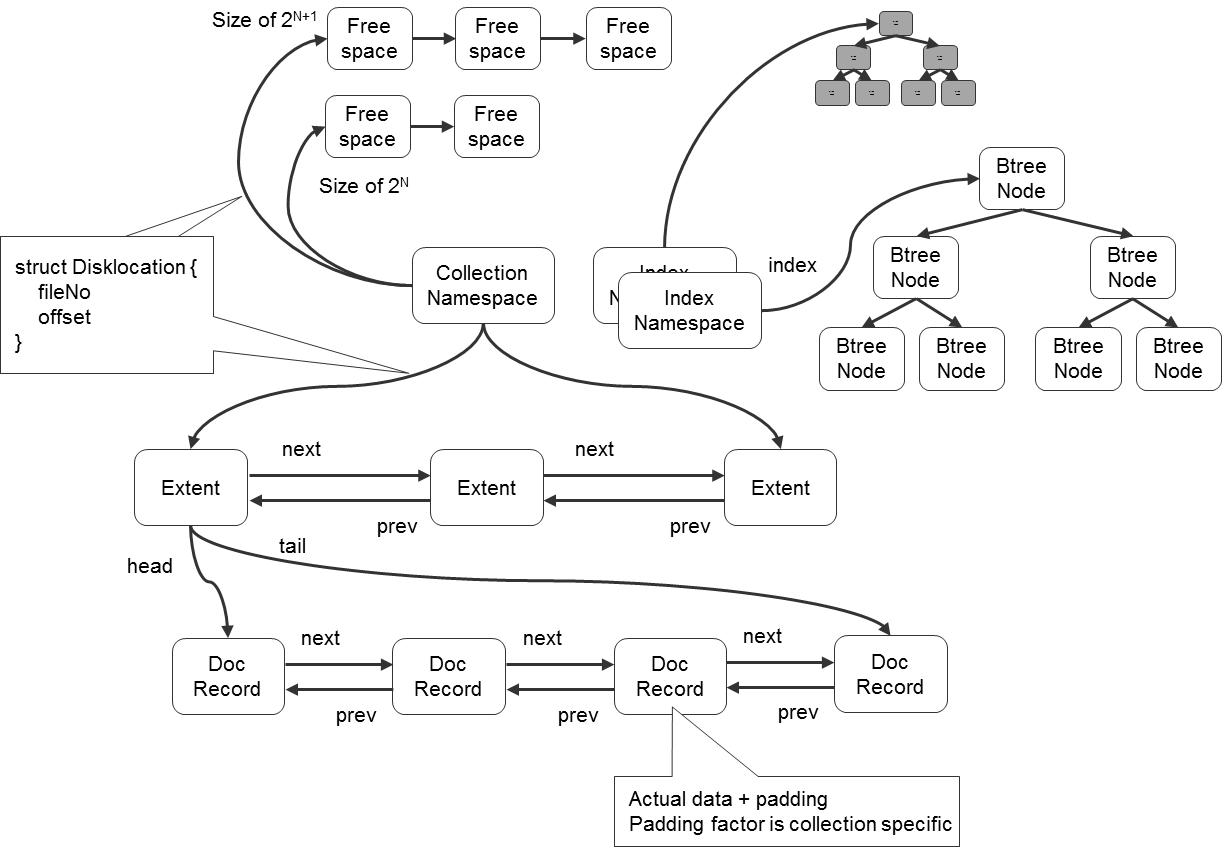
\includegraphics[width=0.8\textwidth]{images/mongodb-storage-structure.png}
\centering
\caption{MongoDB Storage Structure}
%https://haifengl.files.wordpress.com/2014/05/b1912-p1.png?w=1222&h=848
\end{figure}

The data and space are mainly organized through doubly-linked-list. Each collection of data is organized in a linked list of extents. Each extent points to a head/tail of another linked list of documents (up to 16MB). Data files may get fragmented over time because of updates and deletes. It especially gets worse if documents have various sizes. Fragmentation wastes memory and disk space and also make writes scattered and slower. MongoDB provides compact command for defragmentation.

Changes in memory mapped files are flushed to disk every 60 seconds. MongoDB uses write ahead logging to an on-disk journal (called oplog) to guarantee write operation durability and to provide crash resiliency. The write-ahead log is committed every 100 milliseconds by default (configurable with -journalCommitInterval). So the maximum data loss is 100 ms on a hard crash. To achieve durability (i.e. data written to the on-disk journal when acked), you can use the ``j'' option in write concern (discussed in details later).

MongoDB uses a readers-writer lock that allows concurrent read access to a database but exclusive write access to a single write operation. Before version 2.2, this lock was implemented on a per-mongod basis. Since version 2.2, the lock has been implemented at the database level. In a properly designed schema a write will hold the lock for approximately 10 microseconds. If a slow-running operation is predicted (e.g., a document or an index entry will need to be paged in from disk), then that operation will yield the write lock. In version 3.0, the MMAPv1 storage engine adds support for collection-level locking by default.

\subsubsection{WiredTiger}
WiredTiger \cite{WiredTiger}\index{MongoDB!WiredTiger} is introduced in version 3.0 to make MongoDB burn through write-heavy workloads and be more resource efficient.
WiredTiger is a high performance, scalable, transactional key-value store. WiredTiger takes full advantage of modern, multi-core servers with access to large amounts of RAM. WiredTiger's transactions use optimistic concurrency control algorithms that avoid the bottleneck of a centralized lock manager. WiredTiger offers both LSM tree and B-tree engines. To minimize on-disk overhead and I/O, WiredTiger uses compact file formats and compression.
The WiredTiger storage engine provides document-level locking.

\subsection{Cluster Architecture}

Although MongoDB can run as a single instance, it is often configured in a cluster environment to provide scalability and high availability.

\subsection{Replic Set}
High availability is achieved in MongoDB via Replica Set, which provides data redundancy across multiple physical servers, including a single primary as well as multiple secondaries that replicate the primary's oplog and apply the operations to their data sets. The primary accepts all write operations from clients and therefore provides strict consistency. 

By default, clients also read from the primary. To improve read throughput, clients can specify a read preference to send read operations to secondaries. With ``nearest'' read preference, the client driver periodically pings the members and will favor issuing queries to the one with lowest latency. Notice that read request is issued to only one node, there is no quorum read or read from multiple nodes. With read preferences, however, the read results may not reflect latest writes because replications are done asynchronously. 

MongoDB allows users to specify write availability in the system, which is called the write concern. Write concern can include the {\em w} option to specify the required number of acknowledgments from replica set before returning, the {\em j} option to require writes to the journal before returning, and {\em wtimeout} option to specify a time limit to prevent write operations from blocking indefinitely. Prior to November 2012, MongoDB's client drivers return when the writes had only entered the client's outgoing queue. Now the default write concern acknowledges writes received by the primary (but before writing to journal), allowing the client to catch network exceptions and duplicate key errors. 

\begin{figure}[t]
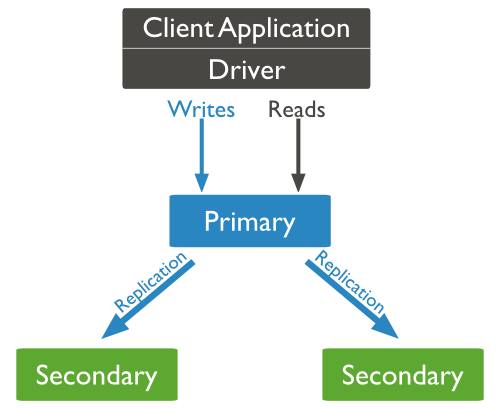
\includegraphics[width=0.8\textwidth]{images/mongodb-replica-set.png}
\centering
\caption{MongoDB Replica Set Structure}
%https://i0.wp.com/docs.mongodb.org/manual/_images/replica-set-read-write-operations-primary.png
\end{figure}

Within the replica set, members are interconnected with each other to exchange heartbeat message. When a primary does not communicate with the other members of the set for more than 10 seconds, the replica set will attempt to select another member to become the new primary. The first secondary that receives a majority of the votes becomes primary. Because of asynchronous replication, the newly elected primary does not necessary having all the latest updates.

Note that a new primary may be elected even if the old one did not crash because of network partition or simply over-loaded primary. In these situations primaries will have accepted write operations that have not replicated to the secondaries after a failover occurs. When the former primary rejoins the replica set and attempts to continue replication as a secondary, the former primary must revert these operations to maintain database consistency across the replica set, which may result in data loss.

\subsection{Sharding}

Although replica set provides data redundancy and potentially load balance of reads with eventually consistency, it does not provide linear scalability for writes since all updates still has to go to the single primary. To load balance writes, MongoDB provides auto-sharding including range-based, hash-based, and tag-award sharding. With sharding, a collection is partitioned into chunks and have chunks distributed across multiple shards.

\begin{figure}[t]
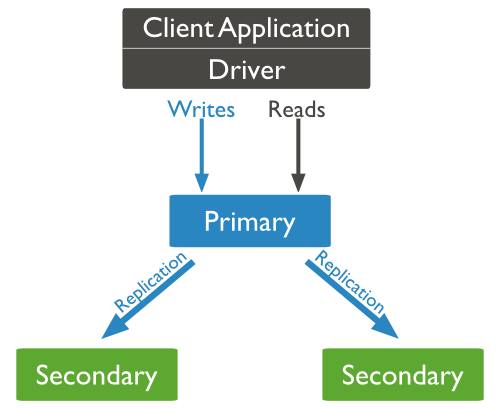
\includegraphics[width=0.8\textwidth]{images/mongodb-replica-set.png}
\centering
\caption{MongoDB Sharding Architecture}
%https://i0.wp.com/docs.mongodb.org/manual/_images/sharded-cluster-production-architecture.png
\end{figure}

A sharded MongoDB cluster consists of the shards, config servers, and routing instances. A shard is a MongoDB instance that holds a subset of a collection's data. Each shard is usually a replica set in production although it can be a single mongod instance. Each config server is a mongod instance that holds metadata about the cluster. The metadata maps chunks to shards. Each router is a mongos instance that routes the reads and writes from applications to the shards. Applications do not access the shards directly.

For writes, the route server will forward the request to the corresponding primary server hosting the chunk whose key range covers the partition key of the document. In case of reads, the routing server will examine whether the partition key is part of the selection criteria and if so will only route the request to the corresponding shard. However, if the partition key is not part of the selection criteria, then the routing server will forward the request to every shard which will perform its local search, and the results will be gathered at the routing server and return to the client.

As chunks grow beyond the specified chunk size a mongos instance will attempt to split the chunk in half. Splits may lead to an uneven distribution of the chunks for a collection across the shards. In such cases, the mongos instances will initiate a round of migrations to redistribute chunks evenly across shards.

\subsection{Summary}
MongoDB is an agile database that allows schemas to change quickly as applications evolve. The JSON-like documents make the integration of data in some applications easier and faster. With careful setup, MongoDB clusters can also provide scalability and high availability.

\chapter[NewSQL]
{NewSQL}

Transactional protected operational workloads are typically deemed mission critical in nature because they help companies make money, touch their customers or prospects, or help them run and operate their business. Typically they have very stringent requirements in terms of response times (sub-second) expectations, transactional data integrity, number of users, concurrency, availability, and data volumes. With the advent of the ``growing internet of things'', the number and types of access devices has driven tremendous transaction and data growth and also changes in the type of data that needs to be captured and utilized as part of these transactions. These next generation operational applications often require multi-structured data types which implies that operational data is evolving rapidly to include a variety of data formats and types of data.

\chapter[Stream Processing]
{Stream Processing}

\section{Storm}

\section{Spark Streaming}


\chapter{Cluster Management}
Large-scale computer clusters are challenging to utilize efficiently. One of the critical tasks of cluster management is to dispatch work for the cluster to perform. The scheduler, assigning jobs to machines, has to take account of a variety of requirements and policies. With the ever-growing size of data, cluster, and workload, the scheduler may become a scalability bottleneck \cite{Schwarzkopf:2013:OFS}.

\section[Mesos]
{Mesos}
\begin{figure}[t]
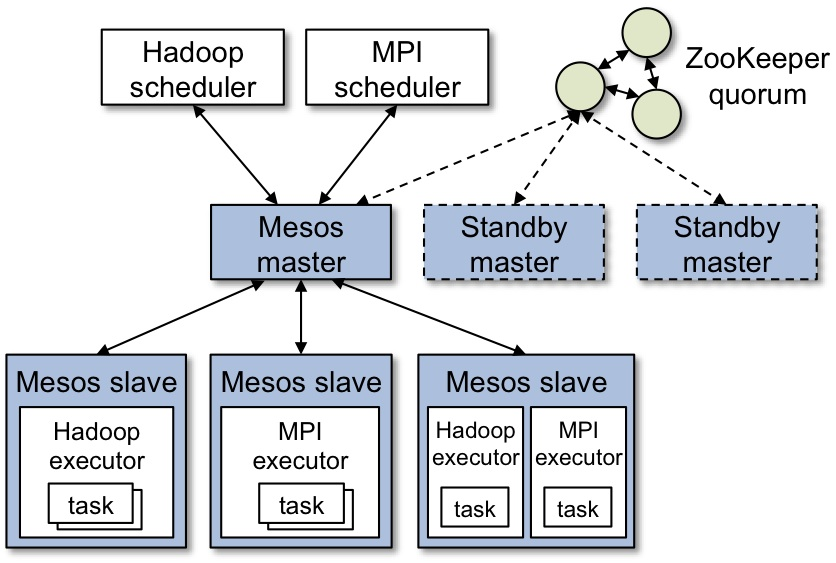
\includegraphics[width=0.8\textwidth]{images/mesos-architecture.jpg}
\centering
\caption{Mesos Architecture}
%http://mesos.apache.org/assets/img/documentation/architecture3.jpg
\end{figure}

Apache Mesos \cite{Hindman:2011:MPF}\index{Mesos} is a cluster resource management software, which gains popularity recently. Mesos uses the master-slave architecture similar to YARN but with a very different design goal. Mesos aims to enable sharing clusters between multiple diverse cluster computing frameworks, such as Hadoop, Spark and MPI. This improves cluster utilization and avoids per-framework data replication.

Mesos introduces a distributed two-level scheduling mechanism \footnote{YARN is a monolithic system and Google's Omega\index{Omega} is a shared state scheduler \cite{Schwarzkopf:2013:OFS}.} and delegates control over scheduling to the frameworks. This allows frameworks to implement diverse approaches to various problems in the cluster and to evolve these solutions independently.

Mesos consists of a master process that manages slave daemons running on each cluster node, and frameworks that run tasks on these slaves.
The master implements resource sharing using through the abstraction {\em resource offer}, which encapsulates a bundle of resources that a framework can allocate on a cluster node to run tasks. The master decides how many resources to offer to each framework according to some (pluggable) policy.

A framework running on top of Mesos consists of two components: a scheduler that registers with the master to be offered resources, and an executor process that is launched on slave nodes to run the framework's tasks.
Resource offers are simple and efficient to implement, allowing Mesos to be highly scalable and robust to failures.

\section[Docker]
{Docker}

\chapter[Graph Processing]
{Graph Processing}

\chapter[Recommendation]
{Recommendation}

\chapter[Text Mining]
{Text Mining}

\chapter[Deep Learning]
{Deep Learning}

%%%%%%%%%%%%%%%%%%%%%%%%%%%%%%%%%%%%%%%%%%%%%%%%%%%%%%%%%%%%%%%%
%% INDEX: Use only one index command set:

%% 1) The default LaTeX Index
\printindex

%% 2) For Topic index and Author index:

% \usepackage{multind}
% \makeindex{topic}
% \makeindex{authors}
% \begin{document}
% ...
% add index terms to your book, ie,
% \index{topic}{A term to go to the topic index}
% \index{authors}{Put this author in the author index}

%% (these are Wiley commands)
%\multiprintindex{topic}{Topic index}
%\multiprintindex{authors}{Author index}

\bibliography{bigdata}

\end{document}
